\documentclass[12pt, a4paper]{article} \setlength{\textheight}{24cm}
\setlength{\textwidth}{16cm} \setlength{\topmargin}{0cm}
\setlength{\evensidemargin}{0cm} \setlength{\oddsidemargin}{0cm}
\usepackage[affil-it]{authblk} \usepackage{graphics}
\usepackage{graphicx} \usepackage{caption} \usepackage{float}
\usepackage[british]{babel} \usepackage{hyperref}
\usepackage{subcaption} \usepackage{algorithm}
\usepackage{algorithmic} \date{}
\begin{document}
\title{Comparison of Several FFT Libraries in C/C++} \author{Philippe
  Gambron \thanks{\texttt{philippe.gambron{@}stfc.ac.uk}}, Sue Thorne
  \thanks{\texttt{sue.thorne{@}stfc.ac.uk}}} \affil{Science and
  Technology Facilities Council, Hartree Centre, Rutherford Appleton
  Laboratory, Harwell Campus, Harwell Oxford, OX11 0QZ, United
  Kingdom}
\maketitle
\begin{abstract}
  We compare the performance of several libraries computing FFTs that
  can be called from C or C++ code. In this work, we consider FFTW,
  MKL, GSL and FFTPACK. A benchmarking method was developed in
  collaboration with CCP-PETMR, which we generalised to ensure that
  this work applied to a wider range of the UK's Computational
  Collaborative Projects and High-End Computing Consortia.
\end{abstract}
\section{Introduction}
Some applications require the computation of the discrete Fourier
transform (DFT) of large datasets. In such cases, the efficiency of
that step can become of critical importance. In this report, we
compare the performance obtained with several libraries that can be
called from C or C++: FFTW \cite{fftw}, MKL \cite{mkl}, GSL \cite{gsl}
and FFTPACK \cite{fftpack}.

\section{The Fast Fourier Transform}

The Fourier transform of a discrete signal $x_j, j=1,\ldots,N,$ at
uniformally d istributed points across a finite domain $[0,N-1]$ in
one dimension is given by:
\begin{equation}\label{fourier} {\cal F}_k=\sum_{j=0}^{N-1} x_j
  e^{-i\frac{2\pi}{N}kj}, \quad k=1,\ldots,N-1.
\end{equation}

We compute it using the Fast Fourier Transform (FFT) method, which
expresses the transform recursively as functions of transforms of more
sparse subsets of the data. The most famous of these methods is the
Cooley-Tukey algorithm \cite{CT}. The procedure can illustrated by
rewriting Equation~\ref{fourier} and splitting the sum into two parts
with one containing the even values of $j$ and the other containing
the odd ones multiplied by a phase factor.
\begin{equation}\label{ct} {\cal
    F}_k=\sum_{j=0}^{N/2-1}x_{2j}e^{-i\frac{2\pi}{N}2jk}+e^{-i\frac{2\pi}{N}k}\sum_{j=0}^{N/2-1}x_{2j+1}e^{-i\frac{2\pi}{N}2jk},
  \quad k=1,\ldots, N-1.
\end{equation}
We can subsequently repeat the procedure by expressing the respective
sums as a function of more sparse transforms till we are left only
with DFTs of a few data points. This dramatically reduces the number
of necessary operations, which become $\cal{O}\left(N\log(N)\right)$
rather than $\cal{O}\left(N^2\right)$.

We also consider Fourier transforms in more dimensions. For example,
in two dimensions, the discrete transform of complex values $z_{j_x
  j_y}$ located on a grid consisting of $N_x \times N_y$ points is
given by:
$$
{\cal F}_{k_x k_y}=\sum_{j_x=0}^{N_x-1} \sum_{j_y=0}^{N_y-1} z_{j_x
  j_y} e^{-i\left(\frac{2\pi}{N_x} j_x k_x+\frac{2\pi}{N_y} j_y
    k_y\right)}, \quad k_x=0,\ldots,N_x-1, k_y=0,\ldots,N_y-1.
$$
The inverse of this transform corresponds to:
$$
{\cal F}_{k_x k_y}=\frac{1}{N_xN_y}\sum_{j_x=0}^{N_x-1}
\sum_{j_y=0}^{N_y-1} z_{j_x j_y} e^{i\left(\frac{2\pi}{N_x} j_x
    k_x+\frac{2\pi}{N_y} j_y k_y\right)}, \quad k_x=0,\ldots,N_x-1,
k_y=0,\ldots,N_y-1.
$$
  
\section{Benchmark}

The benchmark \cite{code} consists in calculating the FFT of a series
of volumes, in 1, 2 or 3 dimensions, of real or complex values. The
purpose was to mimick a problem submitted to us by the CCP PET-MR
collaboration \cite{ccppetmr}, within the Software Outlook initiative
\cite{softwareoutlook}, who needed to take the transform of a series
of square complex images. This example is depicted in Figure
\ref{benchmark} and considered in Section \ref{CCPPETMR}.

\begin{figure}[H]
  \centering
  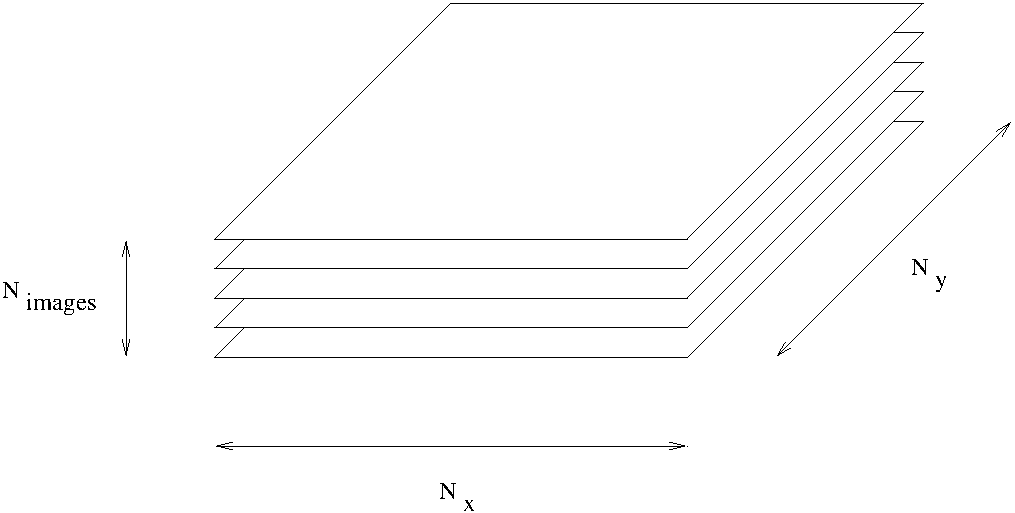
\includegraphics[height=5cm]{benchmark.pdf}
  \caption{The benchmark consists in taking the FFT of several
    images/signals. Each of them is made of real or complex values and
    can be a simple line, a rectangle or a cuboid.}
  \label{benchmark}
\end{figure}

The whole procedure is generalised in Algorithm~\ref{PSEUDOCODE}. We
begin by generating $N_s$ signals (images) in 1, 2 or 3 dimensions.
These can be real or complex values and are sampled at uniformally
distributed points across the domain. For 1D problems, the sampling is
performed at $N$ uniformally spaced points across the domain; in 2D
the sample points $(j_x,j_y)$ are uniformally distributed using a
rectangular mesh with $N_x\times N_y$ points; in 3D the domain is
discretised using a uniform mesh consisting of $N_x\times N_y\times
N_z$ grid points. We then initialise the object performing the FFT and
compute the transform. After this step, we repeat the procedure with
the inverse transform, in order to compute the error. We will measure
the initialisation and execution times of these transforms.
\begin{algorithm}[H]
  \centering
  \begin{algorithmic}
    \FOR {$i = 0,\ldots, N_s-1$} \STATE
    $signal[i]=generate\_signal(N_x [,N_y, N_z])$
    \ENDFOR

    \STATE Initialise $FFT$

    \FOR {$i=0,\ldots,N_s-1$} \STATE $transform[i]=FFT(signal[i])$
    \ENDFOR

    \STATE Initialise $inverse\_FFT$

    \FOR {$i=0,\ldots,N_s$} \STATE
    $inverse\_transform[i]=inverse\_FFT(transform[i])$
    \ENDFOR

    \FOR {$i=0,\ldots,N_s-1$} \STATE $error=error+\left\Vert
      inverse\_transform[i]-signal[i]\right\Vert$
    \ENDFOR
  \end{algorithmic}
  \caption{Pseudocode corresponding to our DFT benchmark}
  \label{PSEUDOCODE}
\end{algorithm}

We vary the number of grid points in our benchmark tests. For most of
the tests, the domains had sides of equal lengths (square or cubic) or
were flattened (rectangle or cuboid). These dimensions could be powers
of 2, products of powers of small integers or prime numbers.

The values appearing in the graphs are the execution time averaged
over 10 runs. A certain number of bumps or slight unexpected features
are apparent. However they were consistently repeated in all our
measurements. This was also confirmed by the standard deviation of our
results, which were always quite small and of the order of a few
percents of the average value. We chose not to display error bars on
our graphs since they were so small that they were barely visible.

\section{Overview of the chosen libraries}
We consider the following libraries computing FFTs: FFTW \cite{fftw},
MKL \cite{mkl}, GSL \cite{gsl} and FFTPACK \cite{fftpack} and
summarise their attributes in Table~\ref{ffttable}). They can perform
complex transforms, real-to-half-complex ones (and conversely) as well
as, in the case of FFTW, real-to-real transforms when the signal is
odd or even. The half-complex output consists in half as many complex
values as there were points in the signal, taking advantage of the
hermiticity of the Fourier transform of a real function.

FFTPACK can compute FFTs in several dimensions but it is written in
FORTRAN and all the C or C++ wrappers we have found only allow
one-dimensional transforms. The GSL library is only designed to work
in one dimension. However, FFTW and MKL can compute FFTs in several
dimensions. They are also capable of working in a parallel way, using
multithreading and MPI.
\begin{table}[H]
  \begin{tabular}{|l||l|l|l|l|l|}
    \hline
    & Type & Dim. & Optimised Radices & Parallelism & Licence \\
    \hline
    \hline
    FFTW & R$\to$H & Any & 2, 3, 5, 7, 11, 13  & Multithreading  & GPL v2\\
    & C$\to$C & & + any with code & MPI &  \\
    &  H$\to$R & &  generator & &  \\
    & R{\scriptsize (odd/even)}$\to$R & & & &  \\
    \hline
    MKL  &  R$\to$H & Any & & Multithreading & Proprietary\\
    & C$\to$C & & & MPI &  \\
    &  H$\to$R & & & &  \\
    \hline
    GSL  &  R$\to$H & 1 & 2, 3, 5, 6, 7 & - & GPL v3\\
    & C$\to$C & & & &  \\
    &  H$\to$R & & & &  \\
    \hline
    FFTPACK  &  R$\to$H  & 1 & & - & GPL v2\\
    {\scriptsize (CASA wrapper)} & C$\to$C & & & &  \\
    &  H$\to$R & & & &  \\
    \hline
  \end{tabular}
  \caption{Overview of the FFT libraries considered. R stands for real, C for complex, and HC for half-complex.}
  \label{ffttable}
\end{table}

\section{Benchmark set-up}
Our benchmark runs were carried out on ARCHER \cite{archer}, the UK
National Supercomputing Service.  It consists of 4920 compute nodes
each containing two 12-core Intel E5-2697 v2 (Ivy Bridge) processors
and at least 64 GB of RAM. The modules \texttt{gcc/7.2.0} and \\
\texttt{intel/17.0.3.191} were loaded. In order to take advantage of
multi-threading, the environment variable \texttt{KMP\_AFFINITY} must
be set to \texttt{disabled}.

Our benchmark was coded in C++ using double-precision reals. More
precisely, we used version 3.3.8 of FFTW, version 17.0.3 of MKL and
version 2.5 of GSL. Note that we used our own version of Boost, FFTW
and GSL because the version of Boost present on the system was lacking
certain libraries and we wanted to use the most recent versions of
FFTW and GSL. The benchmark was compiled with the flags
\texttt{-std=c++1z -O3 -fopenmp -lm -lfftw3 -lfftw3\_threads
  -lgslcblas -lgsl -lboost\_system -lboost\_chrono\\-liomp5
  -lmkl\_core -lmkl\_intel\_thread -lmkl\_intel\_lp64 -lcasa\_scimath
  \\-llapack}.

Since FFTPACK was written in FORTRAN, we have resorted to the C++
wrapper provided by CASA, the radioastronomy package \cite{casa}. This
is straightforward to install on Debian-like systems, such as the one
used by CCP PET-MR in their virtual environment, where CASA can be
installed using the package manager. However, including the headers
and linking with the libraries was not possible with the version of
CASA distributed by the National Radio Astronomy Observatory.  As a
consequence, this was quite difficult to set up on ARCHER and required
the use of libraries provided by an old version of Debian to match
those available on the system. For this reason, it was also necessary
to use an older version of CASA, 2.4.0.


\section{Effect of the domain size in one
  dimension}\label{PERFORMANCE1D}

In this section, we compare the performance of each library, in one
dimension.  Our example corresponds to the pseudocode in
Algorithm~\ref{PSEUDOCODE}. We have used a single signal ($N_s=1$) and
the number of grid points, $N,$ is set to be either a power of 2, an
integer number of the form $2^j\times  3^k\times  5^l\times 7^m$ or a prime number. The
latter are chosen to be close to the corresponding power of 2
(Table~\ref{SIZES1D}).
\begin{table}[H]
  \centering
  \begin{tabular}{|l|l|l|}
    \hline
    \multicolumn{3}{|c|}{$N$}\\
    \hline
    \hline
    Powers of 2 & Product of small integers & primes\\ \hline
    $2^8=256$	 & $2^2\times 3^2\times 5\times 7=210$	     & 257  \\ \hline
    $2^{10}=1024$	 & $2^2\times 3^2\times 5\times 7=1260$	     & 1021  \\ \hline
    $2^{12}=4096$	 & $2\times 3^2\times 5\times 7=4410$	     & 4093 \\ \hline
    $2^{14}=16384$	 & $2\times 3^2\times 5^3\times 7=15750$	     & 16381 \\ \hline
    $2^{16}=65536$	 & $2\times 3^3\times 5^2\times 7^2=66150$      & 65521 \\ \hline
    $2^{18}=262144$	 & $2\times 3\times 5^3\times 7^3=257250$       & 262139 \\ \hline
    $2^{20}=1048576$  & $2\times 3^2\times 5^2\times 7^4=1080450$    & 1048573 \\ \hline
    $2^{22}=4194304$  & $2^2\times 3^2\times 5^2 7^4=4321800$  &	\\ \hline
    $2^{24}=16777216$ & $2^3\times 3^2\times 5^4\times 7^3=15435000$ &	\\ \hline
    $2^{26}=67108864$ & $2^3\times 3^3\times 5^3\times 7^4=64827000$ &\\ \hline
  \end{tabular}
  \caption{Number of points used for the benchmark in one dimension}\label{SIZES1D}
\end{table}


We run our benchmarks with both real and complex values signals and
use the DFT libraries FFTW (Figure~\ref{1DFFTW}), MKL
(Figure~\ref{1DMKL}), GSL (Figure~\ref{1DGSL}) and FFTPACK
(Figure~\ref{1DFFTPACK}). For each library, we compare the effect of
using the different classes of $N.$ We then compare the different
libraries for powers of 2 (Figure~\ref{1DPOW2}). Figure~\ref{1D} compares the libraries for all cases of $N.$ In each of these cases, we have plotted the
wallclock initialisation time and wallclock forward DFT execution
times as a function of $N.$ We will investigate the effect of
parallelism in Section~\ref{PARALLELISM}. As a consequence, for the
moment, we will run all those benchmarks s erially, as a single
process containing a single thread.


\subsection{1D FFTW}
Analysing the performance of FFTW in Figure~\ref{1DFFTW}, the
initialisation time for real input signals is similar for $N$ a power
of 2 and values of $N$ that can be factored into a product of small
integers: for larger values of $N,$ it increases proportionally to a
power of $N.$ For values of $N$ greater than $2^{14},$ the
initialisation times for prime values of $N$ are at least 20 times
higher than the other classes of $N.$ The behaviour of the
initialisation times is different when the signal is complex-valued.
Namely, when $N$ is a power of 2, the initialisation time flattens out
when $N>10^6.$ Initialisation times are faster for complex input
compared to real input: when $N$ can be factored into a product of
small integers, the difference is approximately a factor of 2.
Compairing DFT execution times for real and complex input signals, the
behaviour is very similar but the complex runs are roughly 2 times
slower than when the signal is real-valued and $N$ is a power of 2 or
the product of small integers. When $N$ is prime, the execution times
are almost identical for real and complex signals.

 
\begin{figure}[htb]
  \centering
  \begin{subfigure}{.5\textwidth}
    \centering
    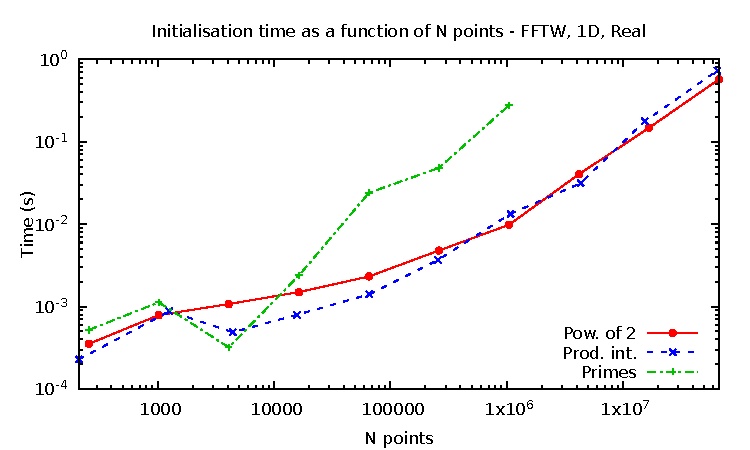
\includegraphics[width=.9\linewidth]{graphs/1d-fftw-init-r.pdf}
    \caption{Initialisation (real)}
    \label{1DFFTWRI}
  \end{subfigure}%
  \begin{subfigure}{.5\textwidth}
    \centering
    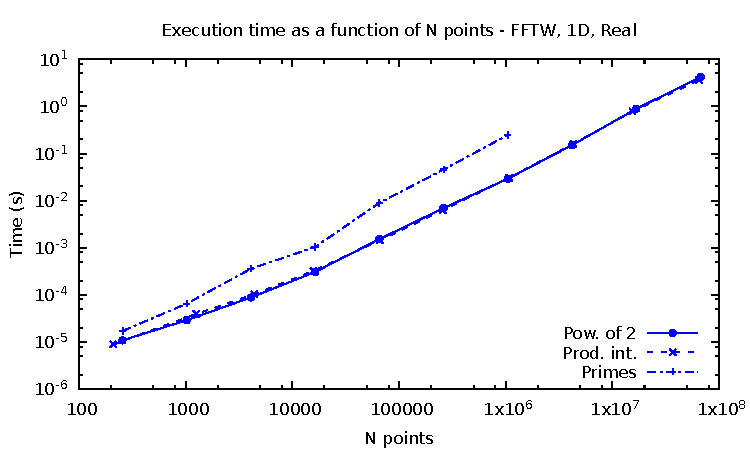
\includegraphics[width=.9\linewidth]{graphs/1d-fftw-exec-r.pdf}
    \caption{Execution (real)}
    \label{1DFFTWR}
  \end{subfigure}\\
  \begin{subfigure}{.5\textwidth}
    \centering
    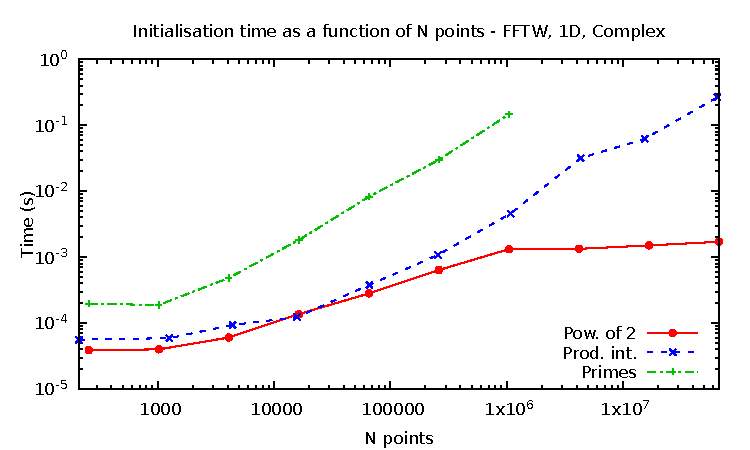
\includegraphics[width=.9\linewidth]{graphs/1d-fftw-init-c.pdf}
    \caption{Initialisation (complex)}
    \label{1DFFTWCI}
  \end{subfigure}%
  \begin{subfigure}{.5\textwidth}
    \centering
    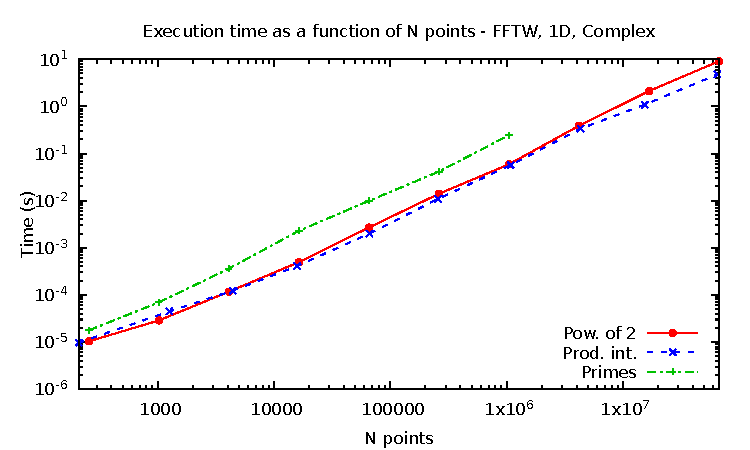
\includegraphics[width=.9\linewidth]{graphs/1d-fftw-exec-c.pdf}
    \caption{Execution (complex)}
    \label{1DFFTWC}
  \end{subfigure}
  \caption{Initialisation and execution times as a function of the
    number of points (1 dimension, FFTW)}
  \label{1DFFTW}
\end{figure}

\subsection{1D MKL}
Figure~\ref{1DMKL} compares the initialisation and DFT execution times
for the MKL library. When the signal is real-valued, there is little
difference in initialisation times for $N$ a power of 2 and $N$ a
product of small integers. Additionally, the initialisation time is
increasing proportionally to a power of the problem size. When $N$ is
prime and the signal is real-valued, there is only a relatively small
increase in intialisation time as the problem size increases. When the
signal contains complex values, the initialisation time is roughly 1.5
times larger for $N$ a product of small integers compared to $N$ being
a power of 2. Additionally, for these cases, the initialisation time
is roughly an order of magnitude smaller than when the signal has real
entries.

The DFT execution times for $N$ a power of 2 or product of small
integers are highly correlated to problem size with execution times
for real input taking roughly twice the time of signals with complex
entries. When $N$ is prime, the DFT execution time is 2.2 times longer
when the signal is real instead of complex.

\begin{figure}[htb]
  \centering
  \begin{subfigure}{.5\textwidth}
    \centering
    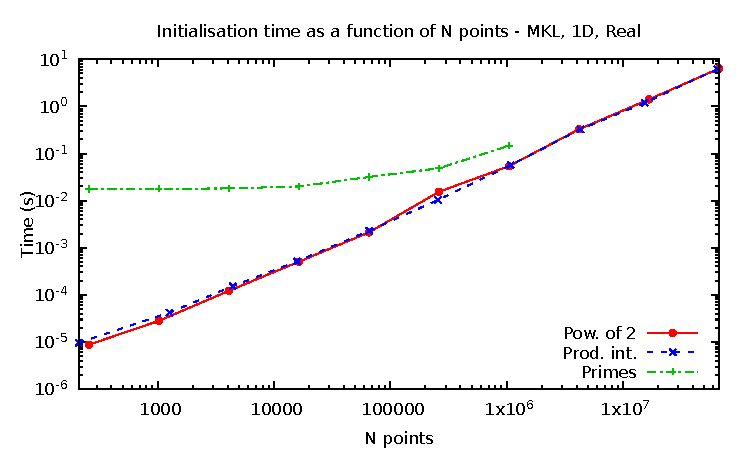
\includegraphics[width=.9\linewidth]{graphs/1d-mkl-init-r.pdf}
    \caption{Initialisation (real)}
    \label{1DMKLRI}
  \end{subfigure}%
  \begin{subfigure}{.5\textwidth}
    \centering
    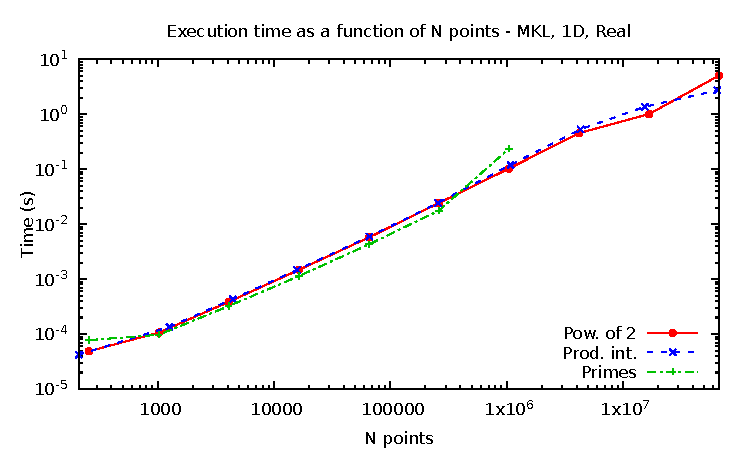
\includegraphics[width=.9\linewidth]{graphs/1d-mkl-exec-r.pdf}
    \caption{Execution (real)}
    \label{1DMKLR}
  \end{subfigure}\\
  \begin{subfigure}{.5\textwidth}
    \centering
    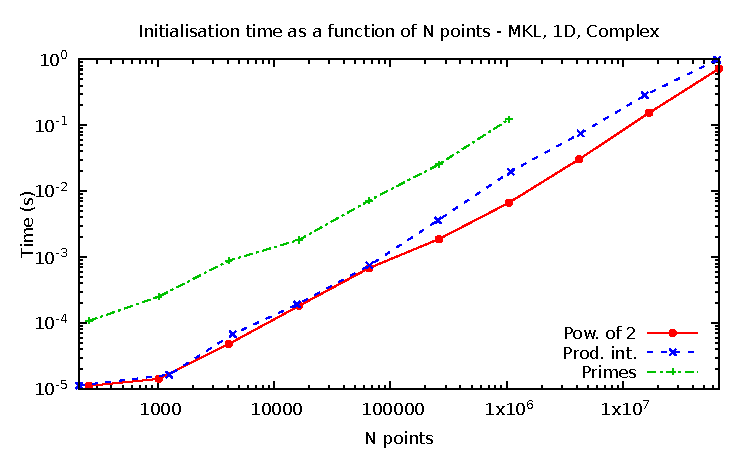
\includegraphics[width=.9\linewidth]{graphs/1d-mkl-init-c.pdf}
    \caption{Initialisation (complex)}
    \label{1DMKLCI}
  \end{subfigure}%
  \begin{subfigure}{.5\textwidth}
    \centering
    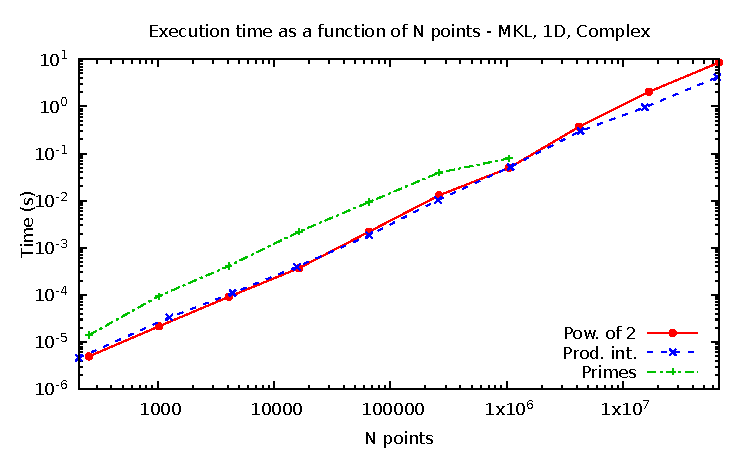
\includegraphics[width=.9\linewidth]{graphs/1d-mkl-exec-c.pdf}
    \caption{Execution (complex)}
    \label{1DMKLC}
  \end{subfigure}\\
  \caption{Initialisation and execution times as a function of the
    number of points (1 dimension, MKL)}
  \label{1DMKL}
\end{figure}

\subsection{1D GSL and FFTPACK}
As with the FFTW and MKL libraries, the initialisation times for GSL,
Figure~\ref{1DGSL}, have differing behaviours for real and complex
signals. For complex signals, there is little difference in
initialisation time for the different classes of $N$ and the time is
proportional to a power of the problem size. When the signal is real,
rather surprisingly, the initialisation time is smallest when $N$ is
prime and the times for the other cases are roughly those for
corresponding complex signals. For real-valued signals with prime
values of $N,$ the DFT execution time increases at a rate proportional
to $N^2.$ For complex signals with $N$ prime, there is a much slower
increase with respect to execution time and the times are roughly 2.5
times those of the other classes of $N$ considered.

The general behaviours of the GSL and FFTPACK (Figure~\ref{1DFFTPACK})
libraries are similar.

\begin{figure}[htb]
  \centering
  \begin{subfigure}{.5\textwidth}
    \centering
    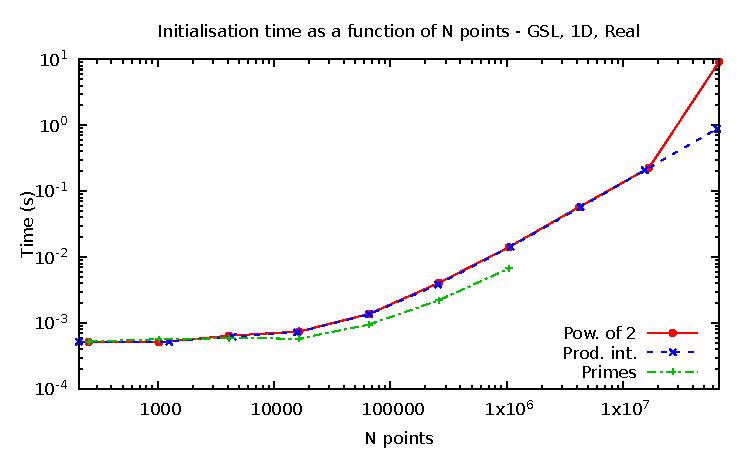
\includegraphics[width=.9\linewidth]{graphs/1d-gsl-init-r.pdf}
    \caption{Initialisation (real)}
    \label{1DGSLRI}
  \end{subfigure}%
  \begin{subfigure}{.5\textwidth}
    \centering
    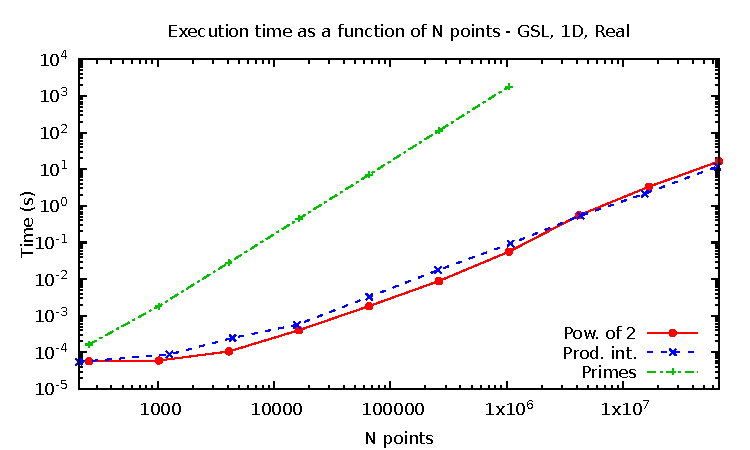
\includegraphics[width=.9\linewidth]{graphs/1d-gsl-exec-r.pdf}
    \caption{Execution (real)}
    \label{1DGSLR}
  \end{subfigure}\\
  \begin{subfigure}{.5\textwidth}
    \centering
    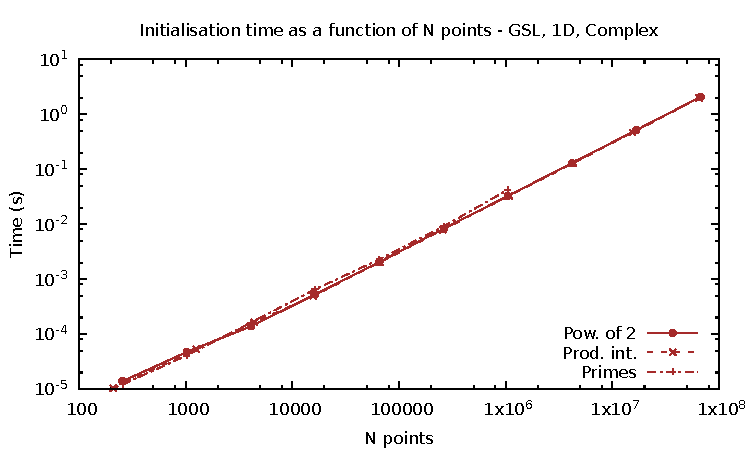
\includegraphics[width=.9\linewidth]{graphs/1d-gsl-init-c.pdf}
    \caption{Initialisation (complex)}
    \label{1DGSLCI}
  \end{subfigure}%
  \begin{subfigure}{.5\textwidth}
    \centering
    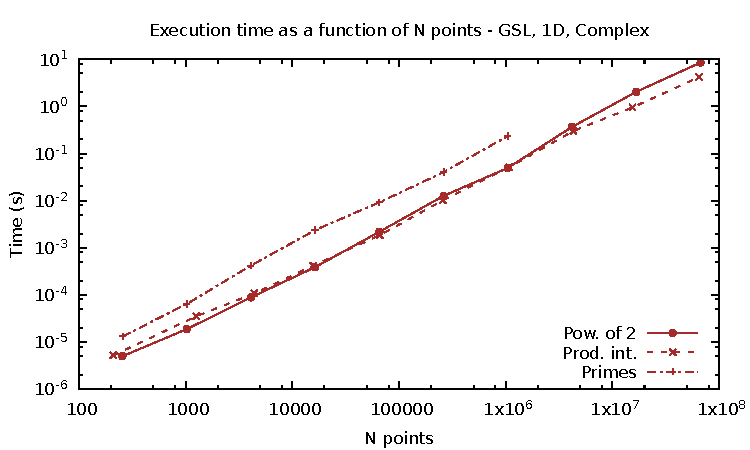
\includegraphics[width=.9\linewidth]{graphs/1d-gsl-exec-c.pdf}
    \caption{Execution (complex)}
    \label{1DGSLC}
  \end{subfigure}
  \caption{Initialisation and execution times as a function of the
    number of points (1 dimension, GSL)}
  \label{1DGSL}
\end{figure}

\begin{figure}[H]
  \centering
  \begin{subfigure}{.5\textwidth}
    \centering
    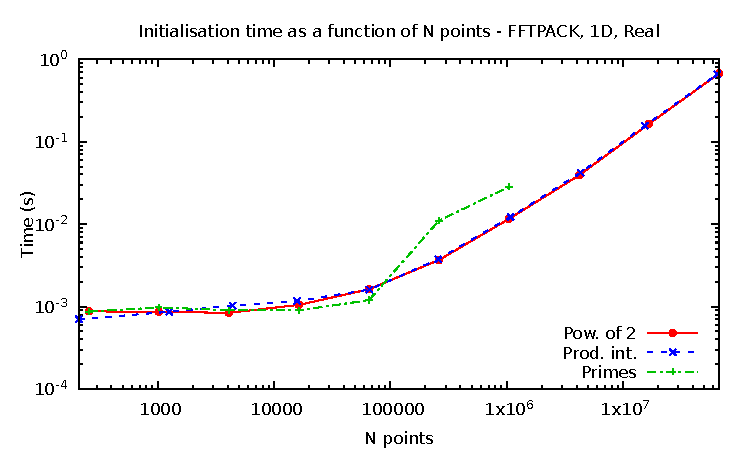
\includegraphics[width=.9\linewidth]{graphs/1d-fftpack-init-r.pdf}
    \caption{Initialisation (real)}
    \label{1DFFTPACKRI}
  \end{subfigure}%
  \begin{subfigure}{.5\textwidth}
    \centering
    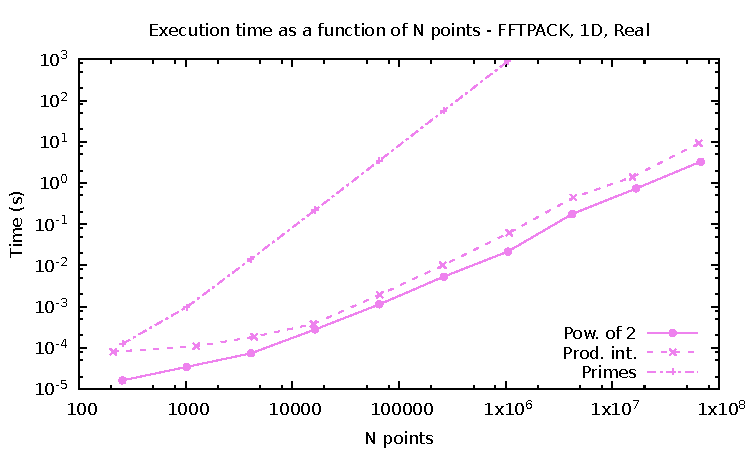
\includegraphics[width=.9\linewidth]{graphs/1d-fftpack-exec-r.pdf}
    \caption{Execution (real)}
    \label{1DFFTPACKR}
  \end{subfigure}\\
  \begin{subfigure}{.5\textwidth}
    \centering
    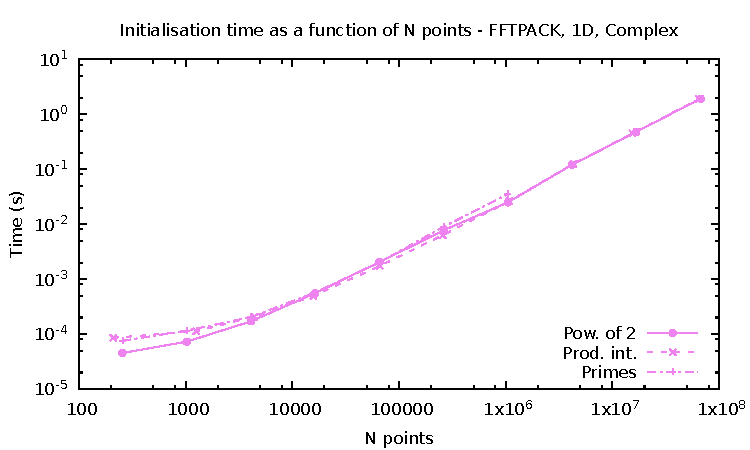
\includegraphics[width=.9\linewidth]{graphs/1d-fftpack-init-c.pdf}
    \caption{Initialisation (complex)}
    \label{1DFFTPACKCI}
  \end{subfigure}%
  \begin{subfigure}{.5\textwidth}
    \centering
    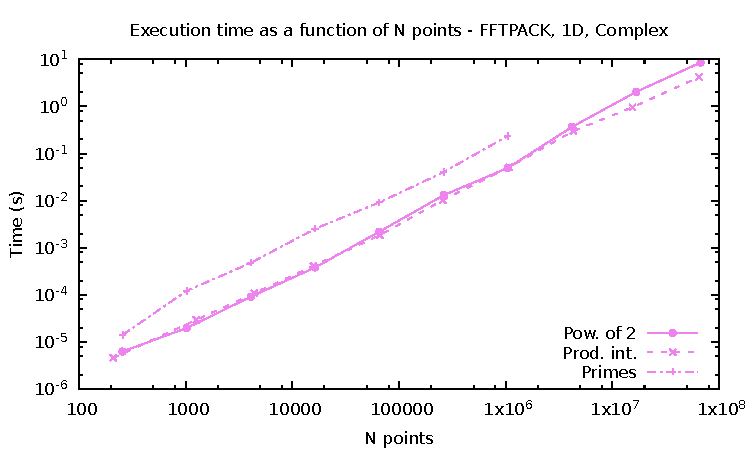
\includegraphics[width=.9\linewidth]{graphs/1d-fftpack-exec-c.pdf}
    \caption{Execution (complex)}
    \label{1DFFTPACKC}
  \end{subfigure}
  \caption{Initialisation and execution times as a function of the
    number of points (1 dimension, FFTPACK)}
  \label{1DFFTPACK}
\end{figure}


\subsection{Comparison libraries for 1D benchmarks}
We also compared the libraries among themselves for powers of 2
(Figure~\ref{1DPOW2}) and all the classes of $N$ considered
(Figure~\ref{1D}). In Table~\ref{Tbl:1D} we provide the initialisation
and DFT execution times for the largest value of prime $N$ considered
and the nearest values of $N$ for the other clasees of $N.$ For large
values of $N$ that are powers of 2 with real input signals, FFTW has
the fastest initialisation time (FFTPACK is similar) whilst FFTPACK
has the fastest DFT execution time with FFTW being approximately 33\%
longer. When $N$ is large and a power of 2 with complex input signals,
all of the libraries have very similar DFT execution times but FFTW
has significantly lower initialisation times.

If $N$ is large and a product of small integers but not a power of 2,
the initialisation time for real input signals is similar for FFTW,
FFTPACK and GSL but the MKL library is (roughly) a factor of four
times larger; for the complex case, FFTW has the best inialisation
time with the GSL library taking about four times longer and the
others taking longer still. Looking at the DFT execution times, FFTW
is fastes for the real case but all of the libraries have similar DFT
execution times in the complex case.


When $N$ is prime, FFTPACK has the fastest initialisation time (both
real and complex cases). However, for real input, the DFT execution
times of GSL and FFTPACK are at least three orders of magnitude larger
than those of FFTW and MKL. If the input signal is complex, MKL has
the best DFT execution times with the others being approximately three
times larger.


Therefore, there is no clear winner but if the input signal is real
and $N$ maybe prime, the GSL and FFTPACK should be avoided.


\begin{figure}[H]
  \centering
  \begin{subfigure}{.5\textwidth}
    \centering
    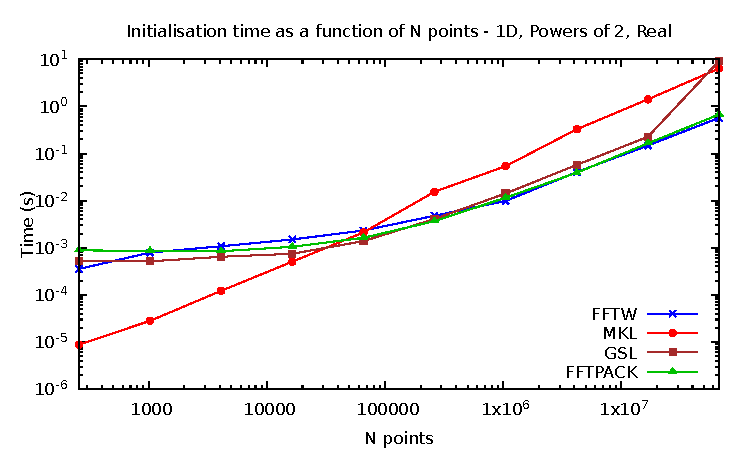
\includegraphics[width=.9\linewidth]{graphs/1d-pow2-init-r.pdf}
    \caption{Initialisation (real)}
    \label{1DPOW2RI}
  \end{subfigure}%
  \begin{subfigure}{.5\textwidth}
    \centering
    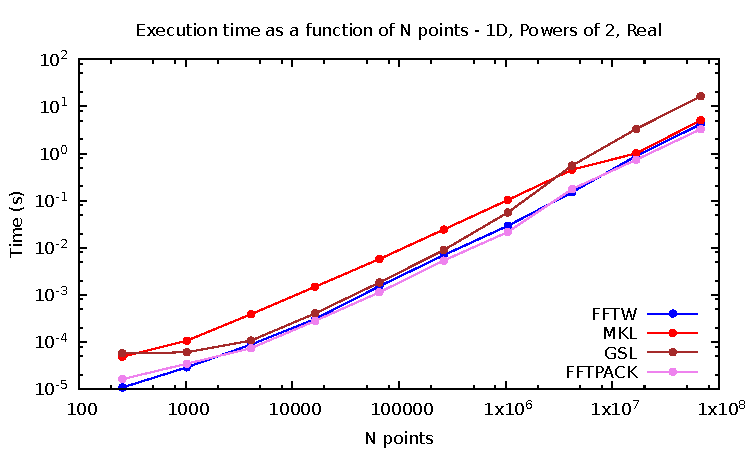
\includegraphics[width=.9\linewidth]{graphs/1d-pow2-exec-r.pdf}
    \caption{Execution (real)}
    \label{1DPOW2R}
  \end{subfigure}\\
  \begin{subfigure}{.5\textwidth}
    \centering
    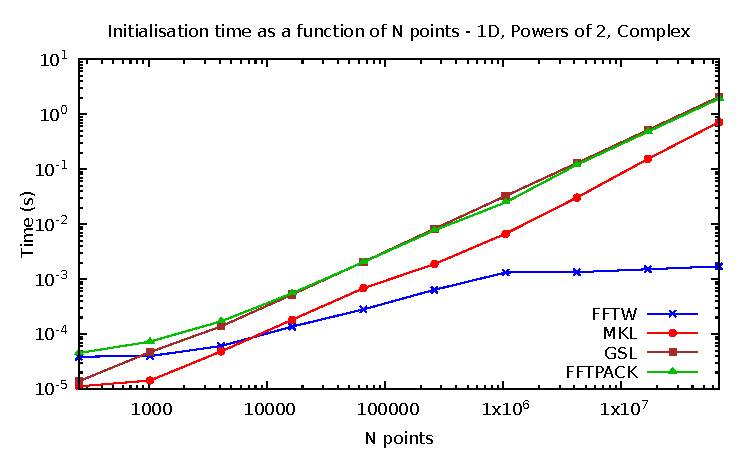
\includegraphics[width=.9\linewidth]{graphs/1d-pow2-init-c.pdf}
    \caption{Initialisation (complex)}
    \label{1DPOW2CI}
  \end{subfigure}%
  \begin{subfigure}{.5\textwidth}
    \centering
    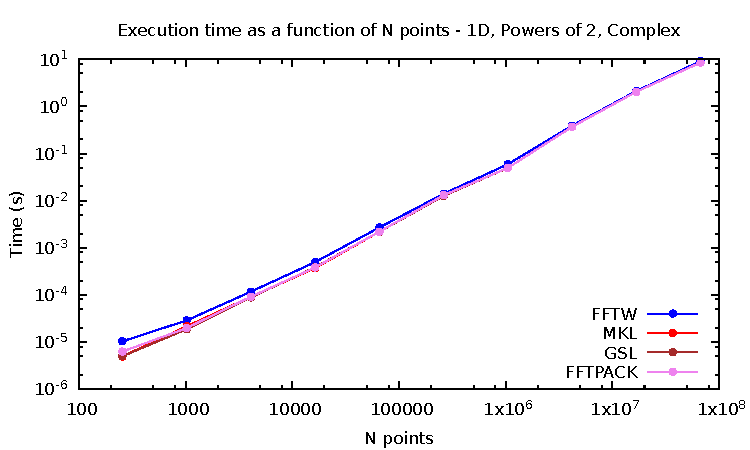
\includegraphics[width=.9\linewidth]{graphs/1d-pow2-exec-c.pdf}
    \caption{Execution (complex)}
    \label{1DPOW2C}
  \end{subfigure}
  \caption{Initialisation and execution times as a function of the
    number of points (1 dimension, powers of 2)}
  \label{1DPOW2}
\end{figure}

\begin{figure}[H]
  \centering
  \begin{subfigure}{.5\textwidth}
    \centering
    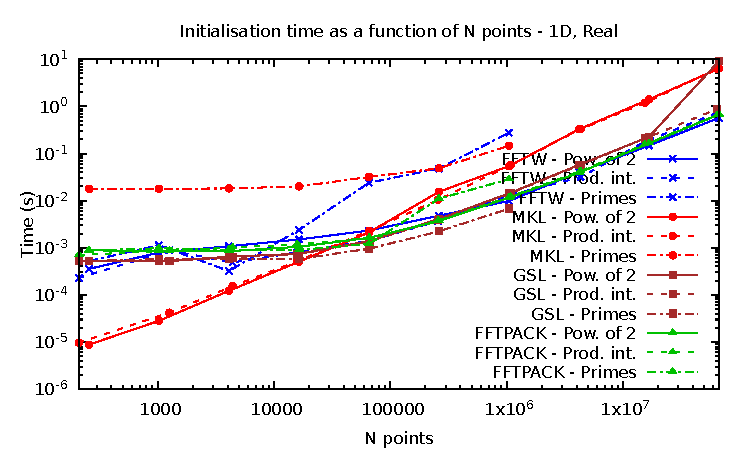
\includegraphics[width=.9\linewidth]{graphs/1d-init-r.pdf}
    \caption{Initialisation (real)}
    \label{1DRI}
  \end{subfigure}%
  \begin{subfigure}{.5\textwidth} \centering
    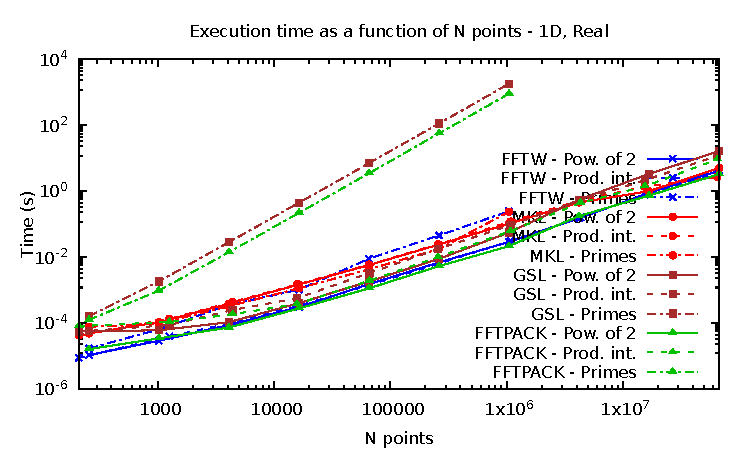
\includegraphics[width=.9\linewidth]{graphs/1d-exec-r.pdf}
    \caption{Execution (real)}
    \label{1DR}
  \end{subfigure}\\
  \begin{subfigure}{.5\textwidth}
    \centering
    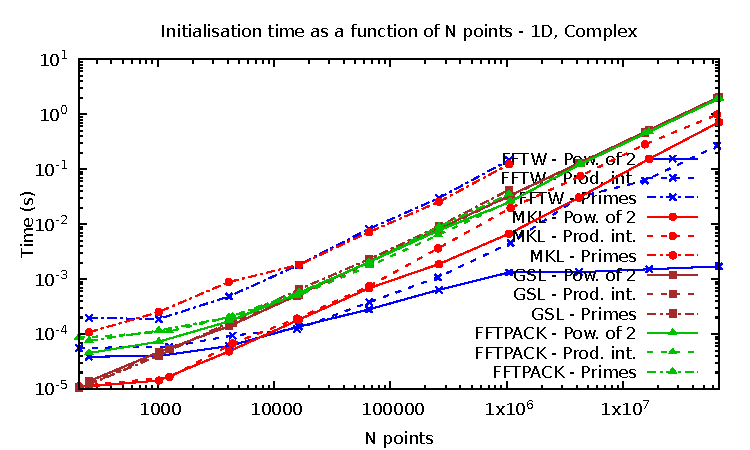
\includegraphics[width=.9\linewidth]{graphs/1d-init-c.pdf}
    \caption{Initialisation (complex)}
    \label{1DCI}
  \end{subfigure}%
  \begin{subfigure}{.5\textwidth}
    \centering
    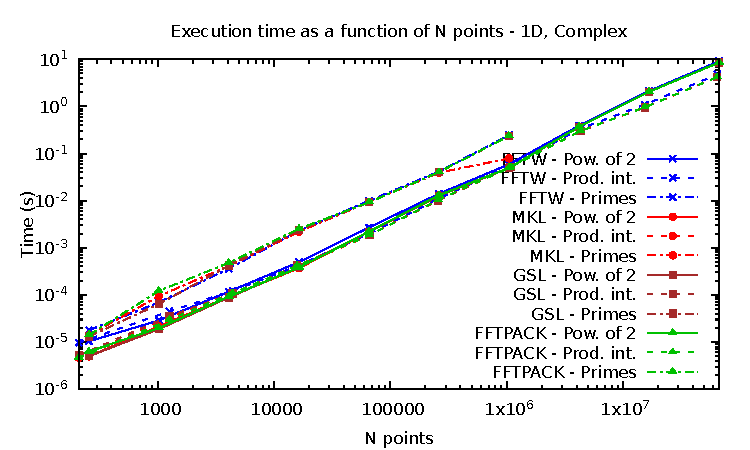
\includegraphics[width=.9\linewidth]{graphs/1d-exec-c.pdf}
    \caption{Execution (complex)}
    \label{1DC}
  \end{subfigure}
  \caption{Initialisation and execution times as a function of the
    number of points (1 dimension)}
  \label{1D}
\end{figure}

\begin{small}
  \begin{table}[H]
    \centering
    \begin{tabular}{|rr|rrrr|rrrr|}
      \hline
      \multicolumn{2}{|c|}{ }& \multicolumn{4}{|c|}{INIT } & \multicolumn{4}{|c|}{DFT }  \\
      $N$ & R/C & FFTW & MKL & GSL & FFTPACK & FFTW & MKL & GSL & FFTPACK \\
      \hline
      \hline
      1048573 & R & 2.76e-1 & 1.47e-1 & 6.75e-2 & 2.84e-2 & 2.46e-1 & 2.36e-1 & 1.18e+3 & 8.97e+2 \\
      1048576 & R &  9.82e-3 & 5.40e-2 &  1.42e-2 &      1.16e-2 &    2.91e-2 &   1.03e-1 &  5.60e-2 & 2.16e-2 \\ 
      1080450 & R & 1.33e-2 & 5.63e-2  & 1.44e-2  & 1.22e-2  & 3.06e-2 & 1.20e-1 & 9.30e-2 & 9.98e-2  \\  
      \hline
      1048573 & C & 1.47e-1 & 1.23e-1 & 4.22e-2 & 3.53e-2 & 2.45e-1 & 7.84e-2 &  2.35e-1 & 2.35e-1 \\
      1048576 & C & 1.32e-3 &  6.69e-3 &      3.26e-2 & 2.49e-2 & 4.93e-2 &  5.90e-2 &  4.94e-2 &   4.94e-2  \\
      1080450 & C &  4.58e-3 & 1.97e-2  & 3.30e-2  & 2.62e-2 & 5.63e-2 & 5.20e-2 & 5.13e-2 & 5.15e-2 \\
      \hline
    \end{tabular}
    \caption{Comparision of average initialisation and DFT execution times for FFTW, MKL GSL and FFTPACK.}\label{Tbl:1D}
  \end{table}
\end{small}

\section{Effect of the domain size in two dimensions}\label{PERFORMANCE2D}

In this section, we measure the performance obtained in two dimensions
following the same procedure as in Section~\ref{PERFORMANCE1D}.
However, only FFTW and MKL work in this case (Figure~\ref{2DFFTW} and
\ref{2DMKL}). In this section, we only consider a square domain. We
will consider asymmetrical domains in Section~\ref{FLATNESS}.

We compare the performance obtained with numbers of points that are a
power of 2, the product of powers of small integers or a prime number.
These numbers are chosen as in Section~\ref{PERFORMANCE1D} and we
endeavoured make the total number of points vary within a similar
range. The dimensions we chose are given in the Table~\ref{SIZES2D}.

\begin{table}[H]
  \centering
  \begin{tabular}{|l|l|l|}
    \hline
    \multicolumn{3}{|c|}{$N_x=N_y=N$}\\
    \hline
    \hline
    Powers of 2 & Product of Small Integers & Primes\\ \hline
    $2^9=512$ & $2^3\times 3^2\times 7=504$ & 509\\ \hline
    $2^{10}=1024$ & $3\times 7^3=1029$ & 1021\\ \hline
    $2^{11}=2048$ & $2\times 3\times 7^3=2058$ & 2027\\ \hline
    $2^{12}=4096$ & $2^2\times 3\times 7^3=4116$ & 4049\\ \hline
    $2^{13}=8192$ & $2^3\times 3\times 7^3=8232$ & 8123\\ \hline
  \end{tabular}
  \caption{Number of points on the side of the square}\label{SIZES2D}
\end{table}

\subsection{2D FFTW}
In Figure~\ref{2DFFTW}, we observe that the initialisation time
behavoiur with respect to $N$ differs depending on whether the input
signal is real or complex. For $N$ a power of 2, the initialisation
time only increases a small amount with respect to increasing $N:$ for
complex signals, the initialisation time is roughly 25\% higher than
when the signal is real. When $N$ is a poroduct of small integers, the
initialisation time is slightly higher than when $N$ is a power of 2
and the complex case is approximately 30\% larger than the real case.
For the three larger values of $N$ with real-valued signals, the
initialisation time is approximately 4 times higher for $N$ prime than
when $N$ is a power of 2; for complex-valued signals there is between
a factor of 2 and 3.5 difference.

The DFT execution time behaviour also differs for real and complex
signals when FFTW is used. In the real case, $N$ being a power of 2
and $N$ being the product of small integers have similar execution
times for prime values of $N$ have execution times that are
approximately 3 times larger. When the signal has complex values and
$N$ is large, the DFT execution times for prime values of $N$ and
powers of 2 are very similar and are roughly 40\% lower than when $N$
is the product of small integers. The complex case with $N$ prime has
DFT times roughly 50\% larger that the real case. For large $N$ that
are powers of 2, the complex case has DFT times that are approximately
a factor of 4.5 larger than when the signal is real.

\begin{figure}[H]
  \centering
  \begin{subfigure}{.5\textwidth}
    \centering
    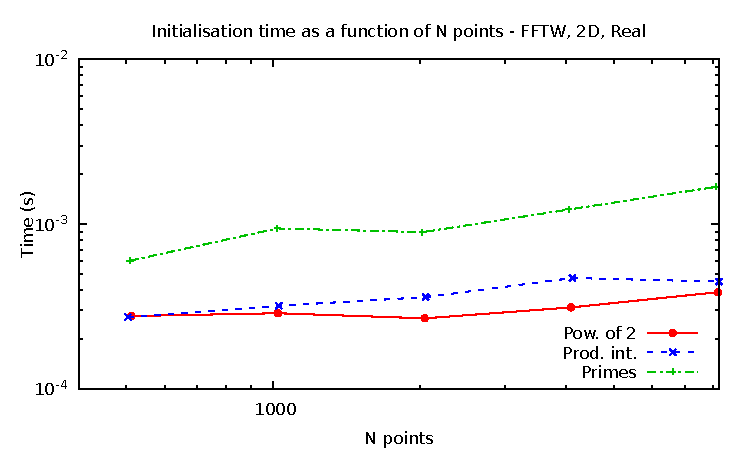
\includegraphics[width=.9\linewidth]{graphs/2d-fftw-init-r.pdf}
    \caption{Initialisation (real)}
    \label{2DFFTWRI}
  \end{subfigure}%
  \begin{subfigure}{.5\textwidth}
    \centering
    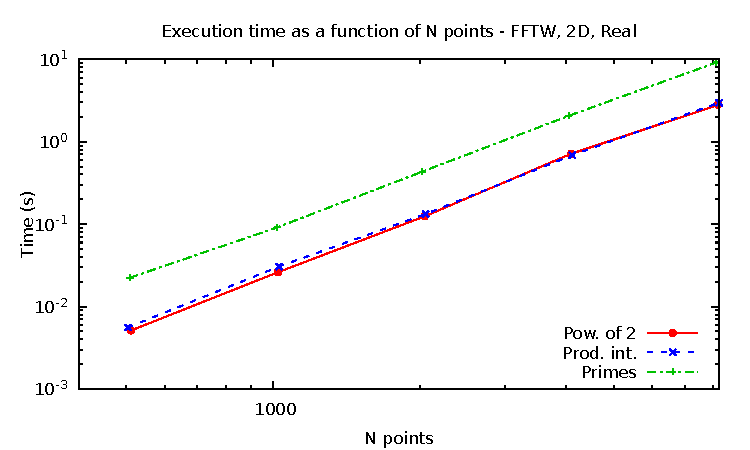
\includegraphics[width=.9\linewidth]{graphs/2d-fftw-exec-r.pdf}
    \caption{Execution (real)}
    \label{2DFFTWR}
  \end{subfigure}\\
  \begin{subfigure}{.5\textwidth}
    \centering
    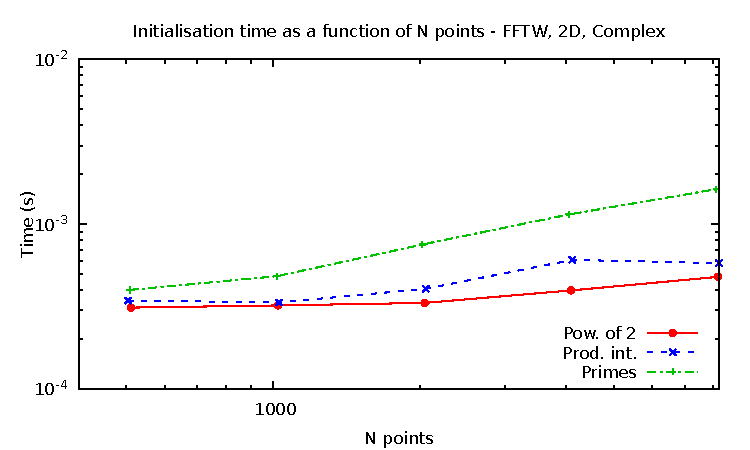
\includegraphics[width=.9\linewidth]{graphs/2d-fftw-init-c.pdf}
    \caption{Initialisation (complex)}
    \label{2DFFTWCI}
  \end{subfigure}%
  \begin{subfigure}{.5\textwidth}
    \centering
    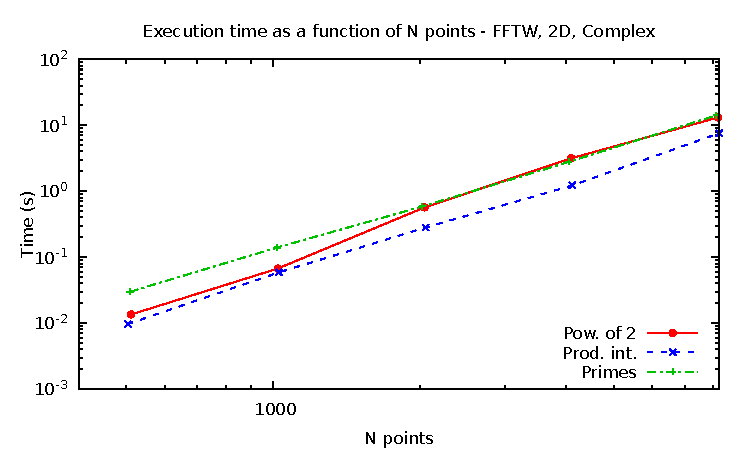
\includegraphics[width=.9\linewidth]{graphs/2d-fftw-exec-c.pdf}
    \caption{Execution (complex)}
    \label{2DFFTWC}
  \end{subfigure}
  \caption{Initialisation and execution times as a function of the
    side of the square (2 dimensions, FFTW)}
  \label{2DFFTW}
\end{figure}



\subsection{2D MKL}
For the MKL library, Figure~\ref{2DMKL}, the initialisation time when
$N$ is prime is significatly larger than the other cases of $N.$
However, when $N$ is a power of 2, the initialisation time is slower
than when $N$ is the product of small integers. When $N$ is a power of
2, the initialisation time is halved if the signal is complex instead
of being real-valued; for $N$ a factor of small integers, the
initialisation time is reduced by roughly a factor of 2.5; for $N$
prime, if is roughly a factor of 1.2 smaller.

The DFT execution time is similar for $N$ being a power of 2 and $N$ a
product of small integers. For real-valued signals, the DFT execution
time increases by roughly a factor of 3 when switching from $N$ being
a power of 2 to $N$ being prime; for complex signals, the time
approximately doubles. Comparing prime values of $N$ with real and
complex signals, there is little difference in DFT execution time.

\begin{figure}[H]
  \centering
  \begin{subfigure}{.5\textwidth}
    \centering
    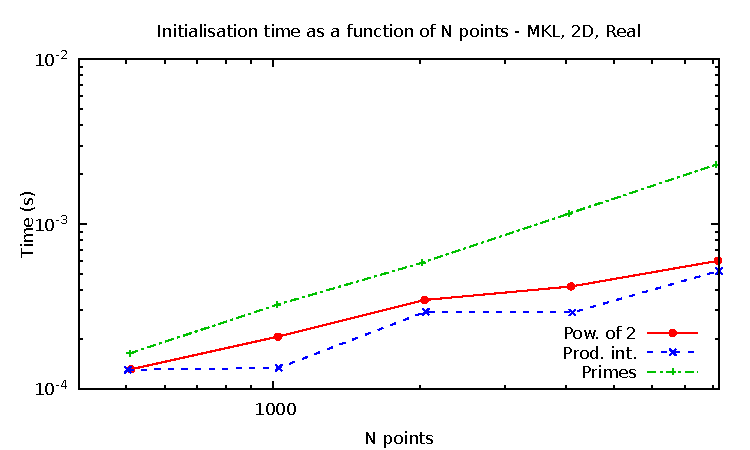
\includegraphics[width=.9\linewidth]{graphs/2d-mkl-init-r.pdf}
    \caption{Initialisation (real)}
    \label{2DMKLRI}
  \end{subfigure}%
  \begin{subfigure}{.5\textwidth}
    \centering
    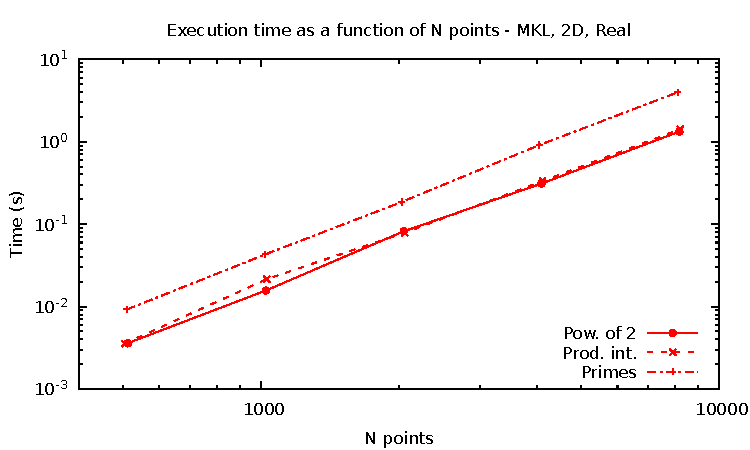
\includegraphics[width=.9\linewidth]{graphs/2d-mkl-exec-r.pdf}
    \caption{Execution (real)}
    \label{2DMKLR}
  \end{subfigure}\\
  \begin{subfigure}{.5\textwidth}
    \centering
    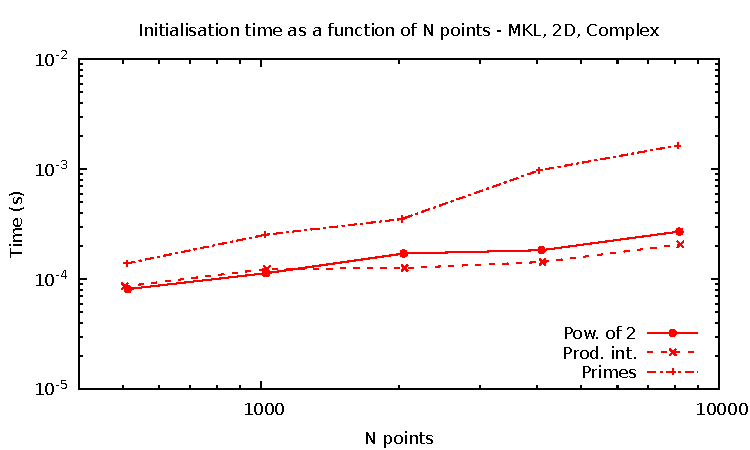
\includegraphics[width=.9\linewidth]{graphs/2d-mkl-init-c.pdf}
    \caption{Initialisation (complex)}
    \label{2DMKLCI}
  \end{subfigure}%
  \begin{subfigure}{.5\textwidth}
    \centering
    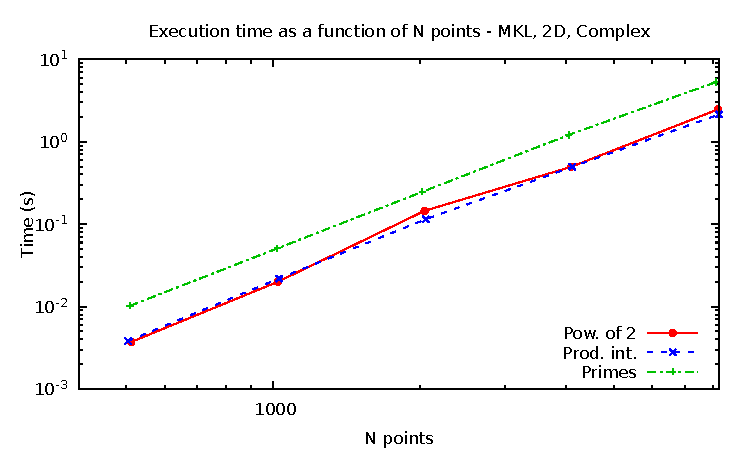
\includegraphics[width=.9\linewidth]{graphs/2d-mkl-exec-c.pdf}
    \caption{Execution (complex)}
    \label{2DMKLC}
  \end{subfigure}
  \caption{Initialisation and execution times as a function of the
    side of the square (2 dimensions, MKL)}
  \label{2DMKL}
\end{figure}






\subsection{2D Library Comparison}
Comparing the two libraries, Figures~\ref{2DPOW2} and \ref{2D}, we
observe that the MKL library generally outperforms FFTW. In
Table~\ref{Tbl:2D}, we provide the average initiation and DFT
execution times for the largest problems in each class of $N$ and
observe that the difference in DFT execution time is significant.


\begin{table}[H]
  \centering
  \begin{tabular}{|rr|rr|rr|}
    \hline
    \multicolumn{2}{|c|}{ }& \multicolumn{2}{|c|}{INIT } & \multicolumn{2}{|c|}{DFT }  \\
     $N$ & R/C & FFTW & MKL & FFTW & MKL \\
    \hline
    \hline
    8123 & R & 1.69e-4 & 2.30e-4 & 9.15 & 3.97 \\
    8192 & R & 3.87e-4 & 5.99e-4 &  2.80 & 1.33  \\ 
    8232 & R & 4.48e-4 & 5.21e-4 & 2.97 & 1.42 \\  
\hline
    8123 & C & 1.63e-4 & 1.64e-4 & 14.1 & 5.30 \\
    8192 & C & 4.79e-4 & 2.71e-4 & 13.1 & 2.47 \\
    8232 & C & 5.80e-4 & 2.07e-4 & 7.56 & 2.15 \\
\hline
  \end{tabular}
  \caption{Comparision of average initialisation and DFT execution times for FFTW and MKL and the largest test problems in each class of $N.$}\label{Tbl:2D}
\end{table}


\begin{figure}[H]
  \centering
  \begin{subfigure}{.5\textwidth}
    \centering
    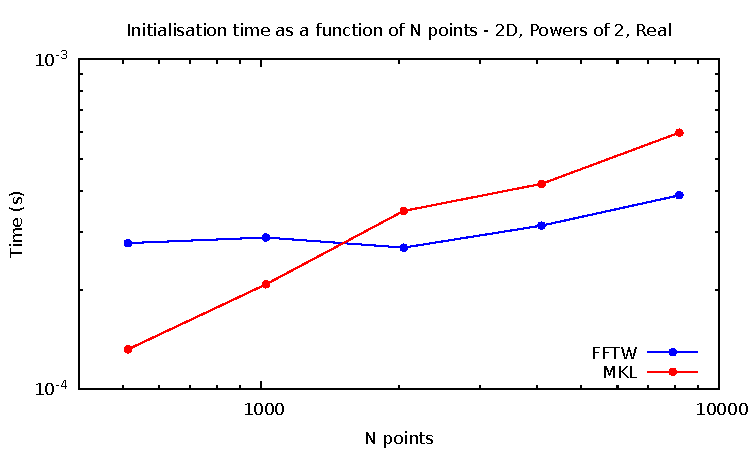
\includegraphics[width=.9\linewidth]{graphs/2d-pow2-init-r.pdf}
    \caption{Initialisation (real)}
    \label{2DPOW2RI}
  \end{subfigure}%
  \begin{subfigure}{.5\textwidth}
    \centering
    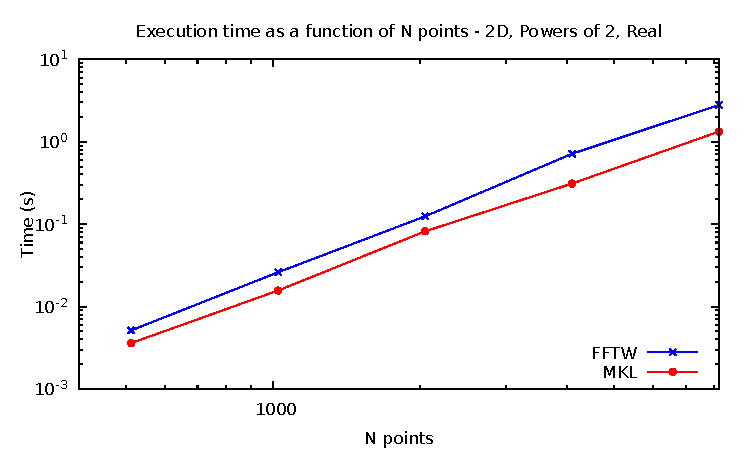
\includegraphics[width=.9\linewidth]{graphs/2d-pow2-exec-r.pdf}
    \caption{Execution (real)}
    \label{2DPOW2R}
  \end{subfigure}\\
  \begin{subfigure}{.5\textwidth}
    \centering
    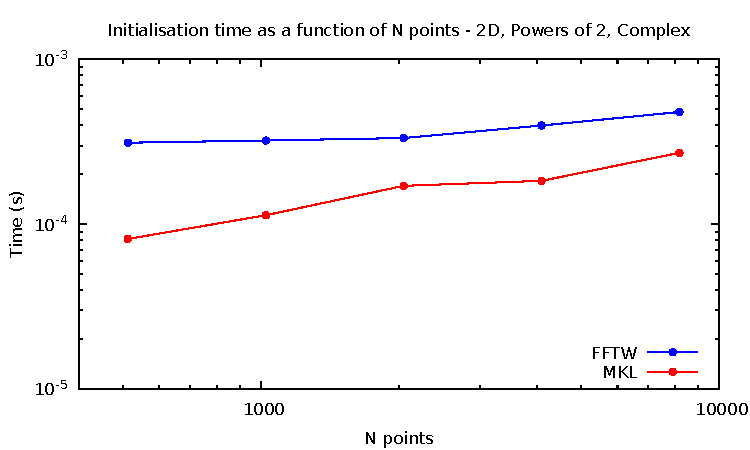
\includegraphics[width=.9\linewidth]{graphs/2d-pow2-init-c.pdf}
    \caption{Initialisation (complex)}
    \label{2DPOW2CI}
  \end{subfigure}%
  \begin{subfigure}{.5\textwidth}
    \centering
    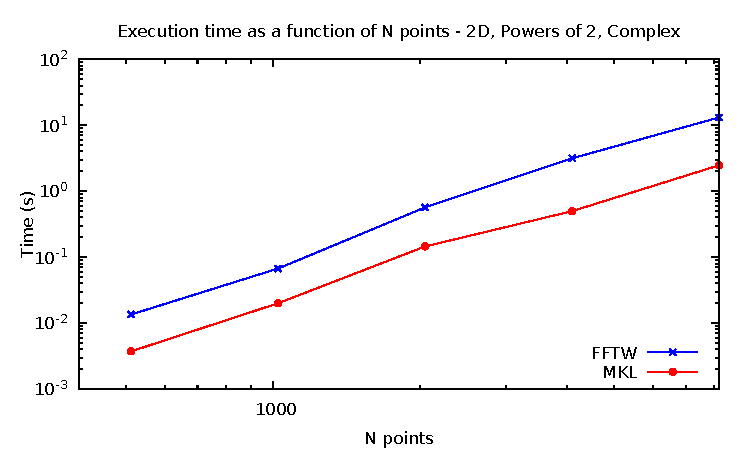
\includegraphics[width=.9\linewidth]{graphs/2d-pow2-exec-c.pdf}
    \caption{Execution (complex)}
    \label{2DPOW2C}
  \end{subfigure}
  \caption{Initialisation and execution times as a function of the
    side of the square (2 dimensions, powers of 2)}
  \label{2DPOW2}
\end{figure}


\begin{figure}[H]
  \centering
  \begin{subfigure}{.5\textwidth}
    \centering
    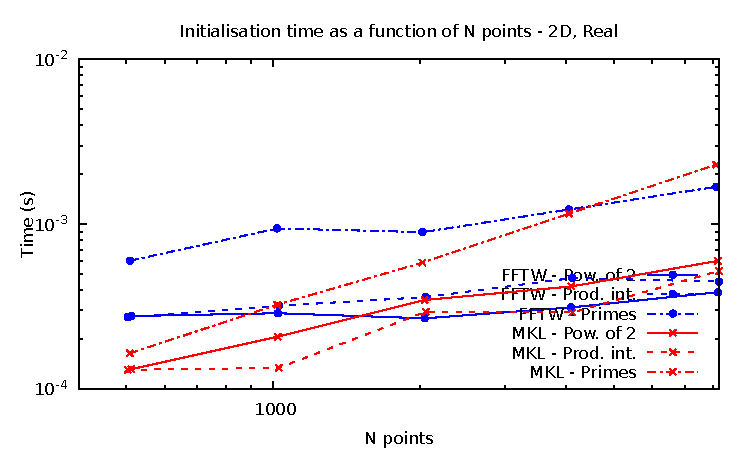
\includegraphics[width=.9\linewidth]{graphs/2d-init-r.pdf}
    \caption{Initialisation (real)}
    \label{2DRI}
  \end{subfigure}%
  \begin{subfigure}{.5\textwidth}
    \centering
    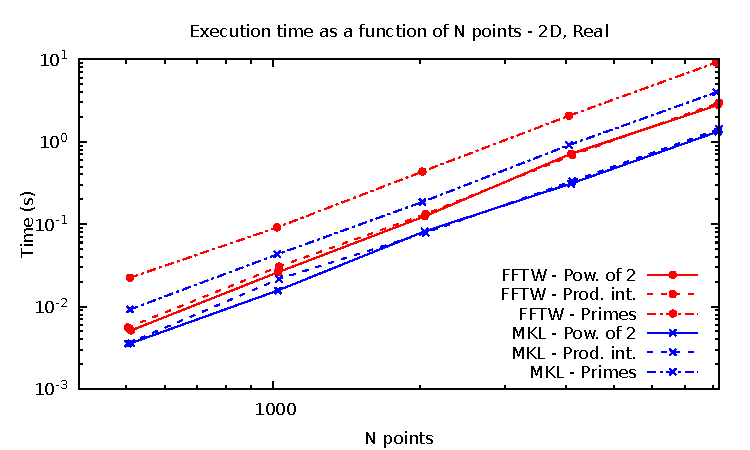
\includegraphics[width=.9\linewidth]{graphs/2d-exec-r.pdf}
    \caption{Execution (real)}
    \label{2DR}
  \end{subfigure}\\
  \begin{subfigure}{.5\textwidth}
    \centering
    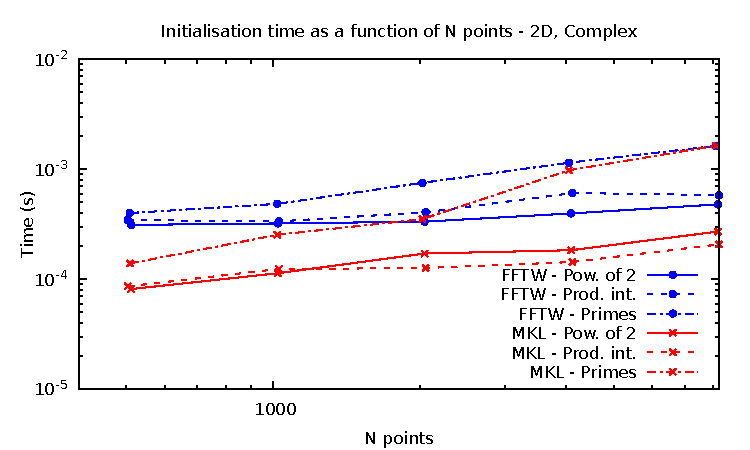
\includegraphics[width=.9\linewidth]{graphs/2d-init-c.pdf}
    \caption{Initialisation (complex)}
    \label{2DCI}
  \end{subfigure}%
  \begin{subfigure}{.5\textwidth}
    \centering
    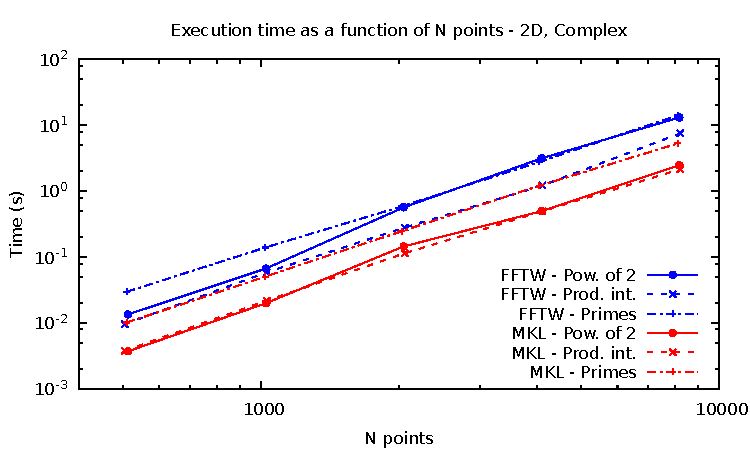
\includegraphics[width=.9\linewidth]{graphs/2d-exec-c.pdf}
    \caption{Execution (complex)}
    \label{2DC}
  \end{subfigure}
  \caption{Initialisation and execution times as a function of the
    side of the square (2 dimensions)}
  \label{2D}
\end{figure}

\section{Effect of the domain size in three  dimensions}\label{PERFORMANCE3D}

We repeat the analysis carried out in Sections \ref{PERFORMANCE1D} and
\ref{PERFORMANCE2D} in three dimensions, on a cubic domain, with the
FFTW and MKL libraries. The number of points considered is given in
Table \ref{SIZES3D}.

\begin{table}[H]
  \centering
  \begin{tabular}{|l|l|l|}
    \hline
    \multicolumn{3}{|c|}{$N_x=N_y=N_z=N$}\\
    \hline
    \hline
    Powers of 2 & Product Small Integers & Primes\\ \hline
    $2^5=32$ & $2\times 3\times 5=30$	& 31\\ \hline
    $2^6=64$ & $2\times 5\times 7=70$	& 61\\ \hline
    $2^7=128$ & $3\times 5\times 7=105$ & 127\\ \hline
    $2^8=256$ & $2\times 3\times 5\ 7=210$ & 257\\ \hline
    $2^9=512$ & $2^2\times 3\times 5\times 7=420$ & 509\\ \hline
  \end{tabular}
  \caption{Number of points on the side of the cube used for the benchmark}\label{SIZES3D}
\end{table}

\subsection{3D FFTW Library}
Results for the FFTW library applied to our 3D benchmark problems are
provided in Figure~\ref{3DFFTW}. We see that the initialisation time
is markedly different when comparing the real and complex cases, with
the real case having initialisation times that are significantly
higher than in the comples case when $N$ is either a power of 2 or the
production of small integers: for the largest size of $N$ considered,
there is a factor of 13 difference when $N$ is a power of 2 and a
factor of 9 difference when $N$ is a product of small integers. For
prime values of $N,$ the difference between initialisation times is
roughly a factor of two with the time for real input initialisation
being larger than that of the complex case.

We also observe that the DFT execution time behaviour differs between
real and complex inputs. For $N$ a power of 2, the DFT time increases
at a faster rate when the input is complex: the ratio increases from
1.8 for the smallest problem size to 7.3 for the largest problem size.
Additionally, for the largest problem size with $N$ a power of 2 and
complex input, the execution time is greater than the other cases $N$
that are similar in size. For real inputs, the DFT execution time is
very similar for $N$ a power of 2 and $N$ the product of small
integers but the execution times is close to three times larger for
$N$ prime.


\begin{figure}[H]
  \centering
  \begin{subfigure}{.5\textwidth}
    \centering
    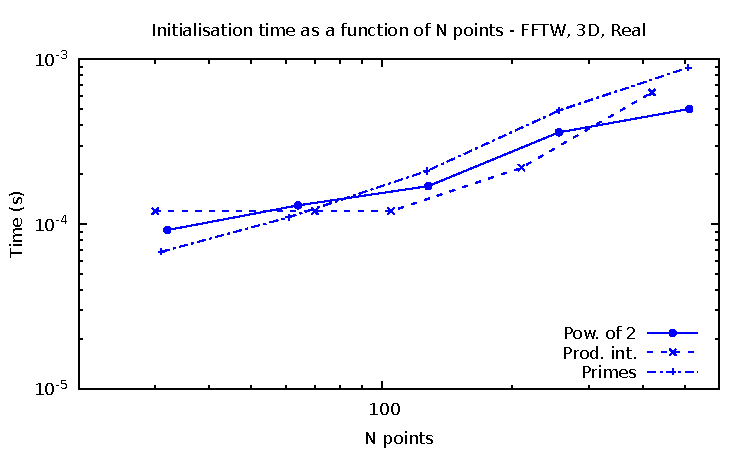
\includegraphics[width=.9\linewidth]{graphs/3d-fftw-init-r.pdf}
    \caption{Initialisation (real)}
    \label{3DFFTWRI}
  \end{subfigure}%
  \begin{subfigure}{.5\textwidth}
    \centering
    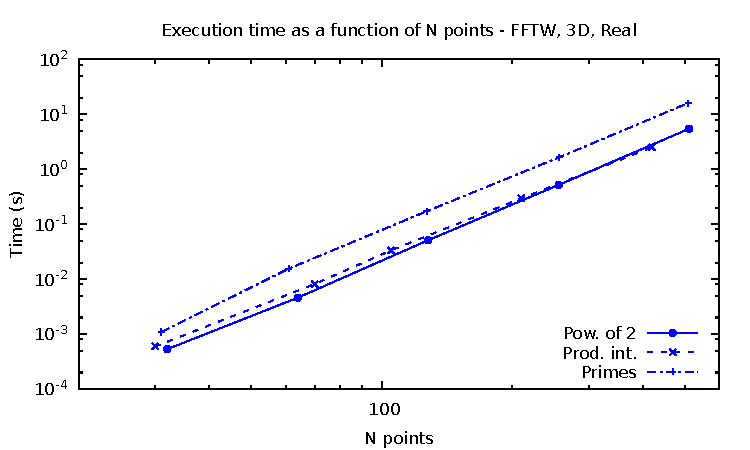
\includegraphics[width=.9\linewidth]{graphs/3d-fftw-exec-r.pdf}
    \caption{Execution (real)}
    \label{3DFFTWR}
  \end{subfigure}\\
  \begin{subfigure}{.5\textwidth}
    \centering
    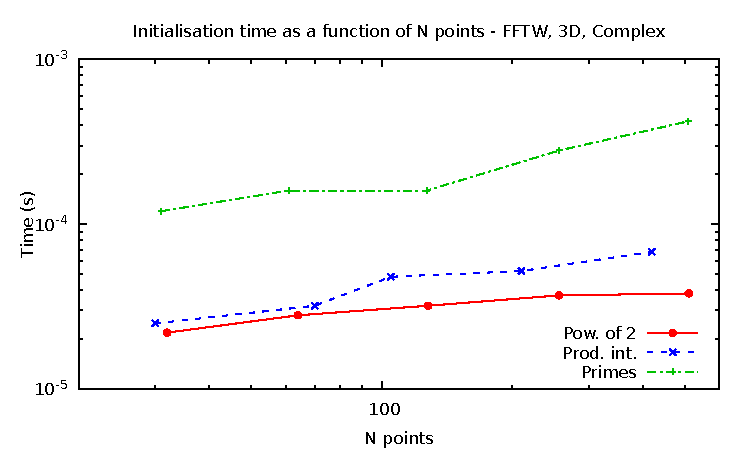
\includegraphics[width=.9\linewidth]{graphs/3d-fftw-init-c.pdf}
    \caption{Initialisation (complex)}
    \label{3DFFTWCI}
  \end{subfigure}%
  \begin{subfigure}{.5\textwidth}
    \centering
    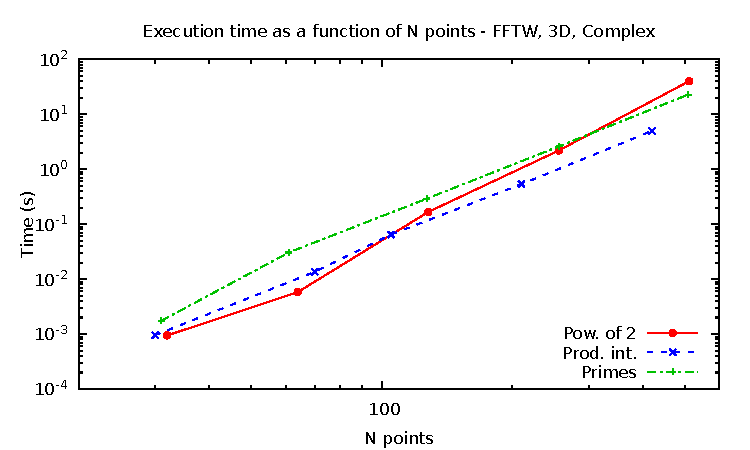
\includegraphics[width=.9\linewidth]{graphs/3d-fftw-exec-c.pdf}
    \caption{Execution (complex)}
    \label{3DFFTWC}
  \end{subfigure}
  \caption{Initialisation and execution times as a function of the
    side of the cube (3 dimensions, FFTW)}
  \label{3DFFTW}
\end{figure}


\subsection{3D MKL Library}
As with FFTW, the initialisation time behaviour with respect to $N$
differs for the real and complex cases. For the real case, the
initialisation time is roughly proportional to a power of $N$ with the
initialisation time for primes taking three times as long as for
comparable values of $N$ that are powers of 2 or the product of small
integers. For the complex case, once $N$ is larger than 100, the
initialisation time starts to fattern off and remains close to
$10^{-4}$ seconds. In this case, prime values of $N$ have
initialisatio ntimes that are roughly twice those for when $N$ is a
power of 1. For $N=2^9,$ the initialisation times is more that four
orders of magnitude smaller that the real case!

The DFT execution time behaviour with respect ot $N$ is similar for
both the real and complex cases and increasing at a rate proportional
to a power of $N.$ The DFT execution time for the real case is, in
general, 40-50\% higher than the complex case. Considering the real
case, the DFT execution time for prime values of $N$ is approximately
triple that of the the other cases of $N$ used within our benchmark
tests. For the complex case, the difference is narrowing as $N$
increases with the ratio being 1.33 for the largest values of $N.$

\begin{figure}[H]
  \centering
  \begin{subfigure}{.5\textwidth}
    \centering
    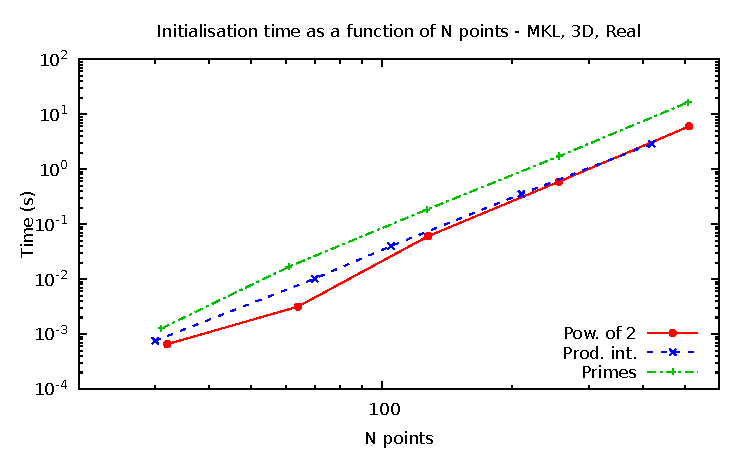
\includegraphics[width=.9\linewidth]{graphs/3d-mkl-init-r.pdf}
    \caption{Initialisation (real)}
    \label{3DMKLRI}
  \end{subfigure}%
  \begin{subfigure}{.5\textwidth}
    \centering
    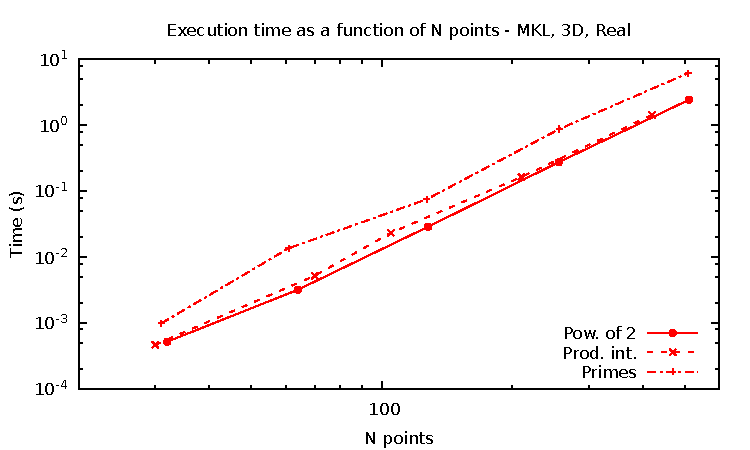
\includegraphics[width=.9\linewidth]{graphs/3d-mkl-exec-r.pdf}
    \caption{Execution (real)}
    \label{3DMKLR}
  \end{subfigure}\\
  \begin{subfigure}{.5\textwidth}
    \centering
    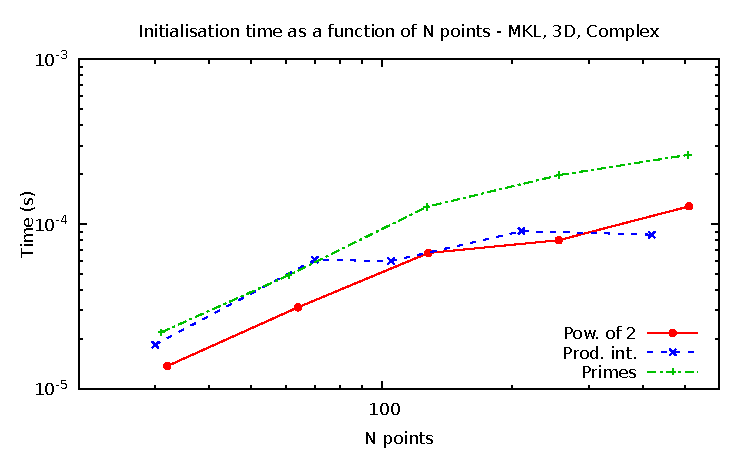
\includegraphics[width=.9\linewidth]{graphs/3d-mkl-init-c.pdf}
    \caption{Initialisation (complex)}
    \label{3DMKLCI}
  \end{subfigure}%
  \begin{subfigure}{.5\textwidth}
    \centering
    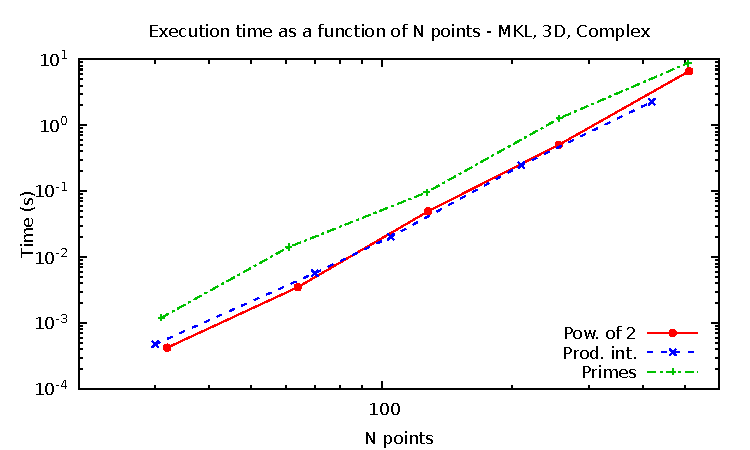
\includegraphics[width=.9\linewidth]{graphs/3d-mkl-exec-c.pdf}
    \caption{Execution (complex)}
    \label{3DMKLC}
  \end{subfigure}
  \caption{Initialisation and execution times as a function of the
    side of the cube (3 dimensions, MKL)}
  \label{3DMKL}
\end{figure}

\subsection{Comparison of libraries for 3D benchmarks}

In Figure~\ref{3DPOW2}, we compare the FFTW and MKL libraries for our
3D benchmark with $N$ a power of 2. For the real case, there is a very
significant difference in the initialisation time: for $N=2^9,$ the
ratio of the MKL library to the FFTW library is 12020. There is a
smaller ratio, 3.38, for the initialisation times in the complex case
with $N$ also equal to $2^9.$ In terms of the DFT execution times, the
MKL library is faster than the FFTW library. In
Table~\ref{Tbl:3DPOW2}, we provide the ratio of the DFT execution
times for differing values of $N$ and observe that there is a greater
difference in execution time in the complex case.

\begin{table}[H]
  \centering
  \begin{tabular}{|r|rrrrr|}
    \hline
    & \multicolumn{5}{|c|}{$N$ }   \\
    R/C & 32 & 64 & 128 & 256 & 512 \\
    \hline
    R & 0.98 & 0.70 & 0.57 & 0.53 & 0.45 \\
    C & 0.45 & 0.60 & 0.29 & 0.23 & 0.16 \\
    \hline
  \end{tabular}
  \caption{Ratio of DFT execution times for 3D benchmark with $N$ a power of 2. Both the real (R) and complex (C) cases for input signals are provided.}\label{Tbl:3DPOW2}
\end{table}

For $N=2^9,$ the time to perform one initialisation and $k$ DFT
calculations will, in general, be larger for the FFTW library for all
$k>2$ (real case) and all $k>0$ (complex case). Thus, unless the user
is doing just one DFT calculation for each initialisation, we would
recommend using the MKL library in the serial case.

\begin{figure}[H]
  \centering
  \begin{subfigure}{.5\textwidth}
    \centering
    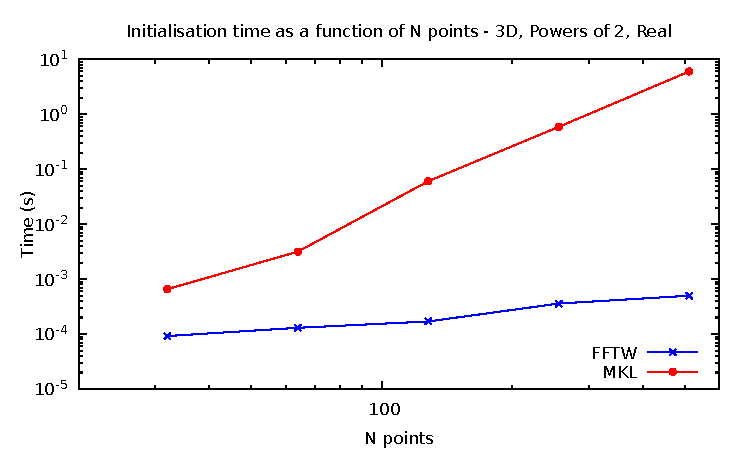
\includegraphics[width=.9\linewidth]{graphs/3d-pow2-init-r.pdf}
    \caption{Initialisation (real)}
    \label{3DPOW2RI}
  \end{subfigure}%
  \begin{subfigure}{.5\textwidth}
    \centering
    \includegraphics[width=.9\linewidth]{graphs/3d-pow2-exec-r.pdf}
    \caption{Execution (real)}
    \label{3DPOW2R}
  \end{subfigure}\\
  \begin{subfigure}{.5\textwidth}
    \centering
    \includegraphics[width=.9\linewidth]{graphs/3d-pow2-init-c.pdf}
    \caption{Initialisation (complex)}
    \label{3DPOW2CI}
  \end{subfigure}%
  \begin{subfigure}{.5\textwidth}
    \centering
    \includegraphics[width=.9\linewidth]{graphs/3d-pow2-exec-c.pdf}
    \caption{Execution (complex)}
    \label{3DPOW2C}
  \end{subfigure}
  \caption{Initialisation and execution times as a function of the
    side of the cube (3 dimensions, powers of 2)}
  \label{3DPOW2}
\end{figure}

The other cases of $N$ considered are included in Figure~\ref{3D}. For
the real case, the MKL initialisation times are always much larger
than those of FFTW. For the complex case and large values of $N,$ the
initialisation times are preferable for FFTW when $N$ is a poroduct of
small integers but not when $N$ is prime. In terms of DFT execution
times, MKL is always preferable. As above, we consider the total time
to perform one initialisation and $k$ DFT calculations. When $N=420$
and the signal is real, the MKL library is generally preferable for
all $k$ greater than 2; for complex input signals, the MKL library is
preferable for all $k>0.$ For $N=509,$ the MKL library is preferable
for the real case when $k>1;$ for complex signals it is preferable for
all $k>0.$

\begin{figure}[H]
  \centering
  \begin{subfigure}{.5\textwidth}
    \centering
    \includegraphics[width=.9\linewidth]{graphs/3d-init-r.pdf}
    \caption{Initialisation (real)}
    \label{3DRI}
  \end{subfigure}%
  \begin{subfigure}{.5\textwidth}
    \centering
    \includegraphics[width=.9\linewidth]{graphs/3d-exec-r.pdf}
    \caption{Execution (real)}
    \label{3DR}
  \end{subfigure}\\
  \begin{subfigure}{.5\textwidth}
    \centering
    \includegraphics[width=.9\linewidth]{graphs/3d-init-c.pdf}
    \caption{Initialisation (complex)}
    \label{3DCI}
  \end{subfigure}%
  \begin{subfigure}{.5\textwidth}
    \centering
    \includegraphics[width=.9\linewidth]{graphs/3d-exec-c.pdf}
    \caption{Execution (complex)}
    \label{3DC}
  \end{subfigure}
  \caption{Initialisation and execution times as a function of the
    side of the cube (3 dimensions)}
  \label{3D}
\end{figure}
\section{Effect of the flatness of the domain}\label{Sec:FLATNESS}

The experiments we carried out in Sections \ref{PERFORMANCE2D} and
\ref{PERFORMANCE3D} were with domains whose dimensions were the same
in all directions, that is, squares or cubes. In this section, we will
study, in three dimensions, the effect of the flatness of the domain
on the performance. We will compute the transform of a signal on a
cuboid containing $512^3$ points stretched in the $z$ direction. The
sides in the $x$ and $y$ directions have identical lengths ($N_x=N_y$)
and the flatness is defined as the ratio between the number of points
in the $z$ and $x$ directions ($N_z/N_x$). The dimensions of the
domains considered appear in Table \ref{FLATNESSDIM}.
\begin{table}[H]
  \centering
  \begin{tabular}{|l|l|l|}
    \hline
    $N_x=N_y$ & $N_z $ & Flatness\\ 
    \hline
    \hline
    512 & 512       & 1\\ \hline
    256 & 2048      & 8\\ \hline
    128 & 8192      & 64\\ \hline
    64  & 32768     & 512\\ \hline
    32  & 131072    & 4096\\ \hline
    16  & 524288    & 32768\\ \hline
    8   & 2097152   & 262144\\ \hline
    4   & 8388608   & 2097152\\ \hline
    2   & 33554432  & 16777216\\ \hline
    1   & 134217728 & 134217728\\ \hline
  \end{tabular}
  \caption{Number of points used for the benchmark in three dimensions}\label{FLATNESSDIM}
\end{table}

We have observed that there is no clear trend in the way the flatness
of the domain affects the performance and conclude that the
performance (in the serial version of each library) depends mostly on the total number of points.

\begin{figure}[H]
  \centering
  \begin{subfigure}{.5\textwidth}
    \centering
    \includegraphics[width=.9\linewidth]{graphs/flatness-r.pdf}
    \caption{Real}
    \label{FLATNESSR}
  \end{subfigure}%
  \begin{subfigure}{.5\textwidth}
    \centering
    \includegraphics[width=.9\linewidth]{graphs/flatness-c.pdf}
    \caption{Complex}
    \label{FLATNESSC}
  \end{subfigure}
  \caption{Execution time as a function of the flatness of the domain
    ($N_y/N_x$), for $N_y=N_z$ (3 dimensions, powers of 2)}
  \label{FLATNESS}
\end{figure}

\section{Parallelism}\label{PARALLELISM}
So far, we have computed FFTs using serial versions of the FFT libraries. 
In this section, we
will investigate the effect of parallelism on the performance
achieved. Only the FFTW and MKL libraries are capable of running in
parallel.

\subsection{Multithreading}\label{MULTITHREADING}
We begin by considering the effect of multithreading on the
computation of the transform of a cube of $512 \times 512 \times 512$
points. We carry out those measurements on a single node of ARCHER
where we can use at most 24 threads and compare FFTW and MKL in
Figure~\ref{3DMTHREAD}. We start by observing that the initialisation
times for the real cases increase for the FFTW libraray as the number
of threads increases but, in comparision, the MKL library's
initialisation times decrease. However, the MKL initialisation times
are at least three orders of magnitude larger than those of FFTW. For
the complex case, the initialisation times for MKL baraely change when
the number of threads differs but, again, the FFTW library has
initialisation times that increase as the number of threads increases
and for the larger number of threads, the initialisation times are
between 16 and 25\% lower than the real case. Comparing the real and
complex cases for the MKL library, the initialisation times are
between three and four orders of magnitude smaller in the complex
case.

With respect to the DFT execution time, the MKL library is nearly
always faster than the FFTW library but the times become similar as
the number of threads increases becasue the FFTW library has better
scaling properties. The complex FFTW DFT execution times are between 2
and 3 times larger than the real case. For the MKL library, the 
corresponding ratios are between 1.8 and 2.5.



\begin{figure}[H]
  \centering
  \begin{subfigure}{.5\textwidth}
    \centering
    \includegraphics[width=.9\linewidth]{graphs/3d-multh-init-r.pdf}
    \caption{Initialisation (real)}
    \label{3DMULTHRI}
  \end{subfigure}%
  \begin{subfigure}{.5\textwidth}
    \centering
    \includegraphics[width=.9\linewidth]{graphs/3d-multh-exec-r.pdf}
    \caption{Execution (real)}
    \label{3DMULTHRE}
  \end{subfigure}\\
  \begin{subfigure}{.5\textwidth}
    \centering
    \includegraphics[width=.9\linewidth]{graphs/3d-multh-init-c.pdf}
    \caption{Initialisation (complex)}
    \label{3DMULTHCI}
  \end{subfigure}%
  \begin{subfigure}{.5\textwidth}
    \centering
    \includegraphics[width=.9\linewidth]{graphs/3d-multh-exec-c.pdf}
    \caption{Execution (complex)}
    \label{3DMULTHCR}
  \end{subfigure}
  \caption{Initialisation and execution times as a function of the
    number of threads (3 dimensions, $512 \times 512\times 512$
    points, FFTW and MKL)}
  \label{3DMTHREAD}
\end{figure}

\subsection{MPI}\label{MPI}
We now turn to studying the effect of the parallelism provided by MPI.
In this case, we used up to 96 processes, corresponding to 4 ARCHER
nodes, each with only a single thread. We carried out the measurements
using a constant number of points on a line ($N_x=16777216$), a square
($N_x=N_y=4096$) and a cube ($N_x=N_y=N_z=256$). We note that the
distributed version of the FFTW library only has interfaces for
complex input signals.


\subsubsection{1D MPI Benchmark Results}
In Figure~\ref{1DMPI}, we compare the distributed versions of the FFTW
and MKL libraries. We start by observing that the MKL library iwht
real input signals has initialisation times that reamin (roughly)
constant as the number of MPI processes increases but the complex
version has initialisation times that decrease slightly (although they
are three orders of magnitude larger than the real case). Moving from
2 to 12 processes, the initialisation times for the FFTW library
steadily decreases but increases again for larger numbers of
processes. The ratio of initialisation times for 1 and 12 MPI
processes is 0.095. Comparing the complex version of the distributed
MKL library with the distributed FFTW library, for the larger number
of MPI processes, the FFTW library's initialisation is about a quarter
of that of MKL.


In terms of DFT execution times, the FFTW library is steadily
decreasing as the number of the processes increases but the MKL
library statys roughly unchanged. Comparing the complex cases, once
more than eight processes are used, FFTW is the favourable library
with respect to the DFT execution time. When 96 MPI processes are
used, the MKL library takes 3.36 times longer than FFTW.

We compare the scalability of the distributed libraries with respect
to the serial version of the libraries in Table~\ref{Tbl:MPI}. The
results show how the DFT execution times can be improved by using the
distributed versions but there is limitations in the scaling
(particularly for the MKL library).

\begin{small}
\begin{table}[H]
  \centering
  \begin{tabular}{|r|rr|rr|rr|}
    \hline
    & \multicolumn{2}{|c|}{FFTW} & \multicolumn{2}{|c|}{MKL(C)} &   \multicolumn{2}{|c|}{MKL(R)}   \\
   $P$ & INIT & DFT & INIT & DFT & INIT & DFT  \\
    \hline
     1 &   4.0481e+1 &   4.4667e-1 &          - &         - &         - &         - \\
   2 &   8.87e+1 &   3.18e-1 &   1.98e+0 &   2.22e-1 &   6.70e-5 &   4.41e-1 \\
   4 &   5.18e+1 &   1.60e-1 &   1.07e+0 &   1.37e-1 &   7.37e-5 &   4.78e-1 \\
   6 &   6.60e+0 &   1.58e-1 &   9.63e-1 &   1.65e-1 &   7.94e-5 &   5.19e-1 \\
   12 &  3.85e+0 &   1.11e-1 &   7.27e-1 &   1.50e-1 &   9.14e-5 &   7.07e-1 \\
   24 &  1.49e+1 &   5.67e-2 &   8.70e-1 &   1.78e-1 &   7.73e-5 &   6.95e-1 \\
   48 &  1.86e+1 &   5.93e-2 &   6.70e-1 &   1.52e-1 &   8.73e-5 &   6.96e-1 \\
   96 &  1.53e+1 &   4.02e-2 &   6.03e-1 &   1.41e-1 &   8.41e-5 &   6.99e-1 \\
    \hline
  \end{tabular}
  \caption{Ratio of initialisation and DFT execution times for 1D MPI benchmark with respect to serial times for different numbers of MPI processes, $P.$ For MKL, the real (R) and complex (C) cases for input signals are provided.}\label{Tbl:MPI}
\end{table}
\end{small}


\begin{figure}[H]
  \centering
  \begin{subfigure}{.5\textwidth}
    \centering
    \includegraphics[width=.9\linewidth]{graphs/mpi-init-1d.pdf}
    \caption{Initialisation}
    \label{1DMPII}
  \end{subfigure}%
  \begin{subfigure}{.5\textwidth}
    \centering
    \includegraphics[width=.9\linewidth]{graphs/mpi-exec-1d.pdf}
    \caption{Execution}
    \label{1DMPIE}
  \end{subfigure}
  \caption{Initialisation and execution times as a function of the
    number of processes (1 dimension)}
  \label{1DMPI}
\end{figure}


\subsubsection{2D MPI Benchmark Results}
We compare the distributed version of FFTW and MKL for our 2D MPI
benchmark in Figure~\ref{2DMPI}. Comparing initialisation times, the
MKL library is significantly faster than the FFTW. For the MKL
library, the real version has initialisation times that increase as
the number of processes increases but they stay roughly constant in
the complex case. However, in general, the initialisation times are
negligible compared to the DFT execution times.

Comparing the DFT execution times, for both libraries, the times are
lower for the real input signal cases: factors of roughly 2.0 and 2.5
for FFTW and MKL, respectively. For our benchmark runs, the MKL
library was faster than FFTW but as the number of processors
increased, the difference became smaller, see
Table~\ref{Tbl:MPI2D}. In Table~\ref{Tbl:MPI2DScale}, we compare the
scalability of the FFTW and MKL distributed libraries with respect to
their serial versions. For FFTW, the distributed version exhibits an
overhead in the initialisation times but this is countered by the DFT
execution times. For the MKL library, there is little different in the
initialisation times when comparing the distributed and serial version
but, for multiple processes, there are gains with respect to the DFT
execution times. However, the FFTW is producing better scalability
trends.




\begin{figure}[H]
  \centering
  \begin{subfigure}{.5\textwidth}
    \centering
    \includegraphics[width=.9\linewidth]{graphs/mpi-init-2d.pdf}
    \caption{Initialisation}
    \label{2DMPII}
  \end{subfigure}%
  \begin{subfigure}{.5\textwidth}
    \centering
    \includegraphics[width=.9\linewidth]{graphs/mpi-exec-2d.pdf}
    \caption{Execution}
    \label{2DMPIE}
  \end{subfigure}
  \caption{Initialisation and execution times as a function of the
    number of processes (2 dimensions)}
  \label{2DMPI}
\end{figure}


\begin{small}
\begin{table}[H]
  \centering
  \begin{tabular}{|r|r|r||}
    \hline
   $P$ & Real & Complex  \\
    \hline
    1 & 2.02 & 1.71   \\
    6 & 1.60 & 1.38  \\
   12 & 1.83 & 1.37  \\
   24 & 1.45 & 1.37  \\
   48 & 1.13 & 1.11  \\
    \hline
  \end{tabular}
  \caption{Ratio of FFTW DFT execution times for 2D MPI benchmark with respect to MKL for different numbers of MPI processes, $P.$ The real and complex cases for input signals are provided.}\label{Tbl:MPI2D}
\end{table}
\end{small}

\begin{small}
\begin{table}[H]
  \centering
  \begin{tabular}{|r|rr|rr|rr|rr|}
    \hline
    & \multicolumn{2}{|c|}{FFTW(C)} & \multicolumn{2}{|c|}{FFTW(R)} & \multicolumn{2}{|c|}{MKL(C)} &   \multicolumn{2}{|c|}{MKL(R)}   \\
   $P$ & INIT & DFT & INIT & DFTg & INIT & DFT & INIT & DFT  \\
    \hline
   1 &   1.37e+1 &   5.40e-1 &   2.25e+1 &   6.98e-1 &   8.93e-1 &   2.00e+0 &   6.15e-1 &   7.94e-1 \\
   2 &   1.75e+1 &   2.40e-1 &   1.21e+1 &   4.23e-1 &  - &  - &   - &  - \\
   4 &   1.86e+1 &   1.37e-1 &   1.29e+1 &   2.82e-1 &  - &  - &    - &  - \\
   6 &   6.20e+0 &   8.63e-2 &   1.25e+1 &   1.76e-1 &   1.00e+0 &   3.95e-1 &   1.01e+0 &   2.52e-1 \\
   8 &  - &  - &   - &  - &   - &  - &   1.09e+0 &   2.18e-1 \\
   12 &   4.83e+0 &   6.27e-2 &   1.22e+1 &   1.44e-1 &   9.44e-1 &   2.90e-1 &   1.22e+0 &   1.82e-1 \\
   16 &  - &  - &  - &  - &  - &  - &    1.23e+0 &   1.54e-1 \\
   24 &   1.50e+1 &   3.12e-2 &   1.52e+1 &   6.77e-2 &   8.68e-1 &   1.45e-1 &   1.16e+0 &   1.07e-1 \\
   48 &   1.60e+1 &   1.83e-2 &   1.50e+1 &   3.30e-2 &   1.02e+0 &   1.05e-1 &   1.43e+0 &   6.68e-2 \\
   96 &   1.73e+1 &   1.37e-2 &   2.27e+1 &   3.29e-2 &  - &  - &  - &  - \\
    \hline
  \end{tabular}
  \caption{Ratio of initialisation and DFT execution times for 2D MPI benchmark with respect to serial times for different numbers of MPI processes, $P.$ For MKL, the real (R) and complex (C) cases for input signals are provided.}\label{Tbl:MPI2DScale}
\end{table}
\end{small}


\subsubsection{3D MPI Benchmark Results}
In Figure~\ref{3DMPI}, we compare the results for our 3D MPI
benchmarks. As with the 2D MPI benchmarks, the DFT execution times are
better for the MKL library but the FFTW library is exhibiting better
scalability properties with respect to the number of processes. In
terms of initialisation times, the MKL library is significantly better
than FFTW and both libraries only exhibit mild changes in
initialisation times as the number of MPI processes increases. As in
the previous subsections, we compare the distributed libraries with
their serial counterparts, Table~\ref{Tbl:MPI3DScale}. We observe how,
in the case of FFTW, the initialisation times has significantly
increased but the DFT execution times are scaling reasonably well with
respect to the number of MPI processes. For MKL, there is little
difference in the initialisation times for the serial and distributed
versions but the scaling properties are not as good as FFTW.

[WHY IS THERE MISSING DATA?]










\begin{figure}[H]
  \centering
  \begin{subfigure}{.5\textwidth}
    \centering
    \includegraphics[width=.9\linewidth]{graphs/mpi-init-3d.pdf}
    \caption{Initialisation}
    \label{3DMPII}
  \end{subfigure}%
  \begin{subfigure}{.5\textwidth}
    \centering
    \includegraphics[width=.9\linewidth]{graphs/mpi-exec-3d.pdf}
    \caption{Execution}
    \label{3DMPIE}
  \end{subfigure}
  \caption{Initialisation and execution times as a function of the
    number of processes (3 dimensions)}
  \label{3DMPI}
\end{figure}


\begin{small}
\begin{table}[H]
  \centering
  \begin{tabular}{|r|rr|rr|rr|rr|}
    \hline
    & \multicolumn{2}{|c|}{FFTW(C)} & \multicolumn{2}{|c|}{FFTW(R)} & \multicolumn{2}{|c|}{MKL(C)} &   \multicolumn{2}{|c|}{MKL(R)}   \\
   $P$ & INIT & DFT & INIT & DFTg & INIT & DFT & INIT & DFT  \\
    \hline
   1 &   7.99e+1 &   8.08e-1 &   8.13e+0 &   7.40e-1 &   8.11e-1 &   1.69e+0 &   9.02e-5 &   8.07e-1 \\
   2 &   1.16e+2 &   2.93e-1 &   1.08e+1 &   4.89e-1 &  - & - & - & - \\
   4 &   1.19e+2 &   1.52e-1 &   1.22e+1 &   2.75e-1 &   9.51e-1 &   4.80e-1 &   1.55e-4 &   3.53e-1 \\
   6 &   8.31e+1 &   1.21e-1 &   6.30e+0 &   2.55e-1 &   7.84e-1 &   3.51e-1 &   1.70e-4 &   2.65e-1 \\
   12 &  5.64e+1 &   8.49e-2 &   6.15e+0 &   1.63e-1 &   1.45e+0 &   2.54e-1 &   1.47e-4 &   1.86e-1 \\
   24 &  1.34e+2 &   3.97e-2 &   7.89e+0 &   9.51e-2 &   1.69e+0 &   1.55e-1 &   9.89e-5 &   1.07e-1 \\
   48 &  2.19e+2 &   3.86e-2 &   1.34e+1 &   7.93e-2 &  - & - & - & - \\
    \hline
  \end{tabular}
  \caption{Ratio of initialisation and DFT execution times for 3D MPI benchmark with respect to serial times for different numbers of MPI processes, $P.$ For MKL, the real (R) and complex (C) cases for input signals are provided.}\label{Tbl:MPI3DScale}
\end{table}
\end{small}



\subsection{MPI and multithreading}\label{MPIMULTH}
We now combine multithreading with MPI in the same conditions as in
Section \ref{MPI}. We increase the number of threads up to the number
of cores on a compute node and subsequently increase the number of
such processes. We carry out this procedure till we use 4 processes,
each consisting of 24 threads. Thus, upto 24 cores, we are really only
assessing the multithreading scalability properties of the distributed
version of the libraries.



\subsubsection{1D MPI+Multithreading Benchmarks}\label{Sec:1DMPIThread}
Again, we note that, in one dimension, FFTW works in a distributed way
only with a complex signal.  We compare the libraries in
Figure~\ref{1DMPIMULTH}) and note that both libraries have relatively
constant initialisation times as the number of cores and processes
increase apart from when we start to incorporate multiple MPI
processes (with 24 cores per process) and then the complex version of
the distributed MKL library exhibits decreasing initialisation times.
Considering the DFT execution times, the MKL libary runs with real
input signals have almost constant times as the number of cores and
processes increase. FFTW also exhibits constant DFT execution times up
until the point at which we use multible MPI processes. However, the
distributed MKL library with complex input signals shows some increase
in DFT execution time as the number of cores increases whilst using
one MPI process. Moving from one to two MPI processes has little
effect on the MPI time but a further increase to four MPI processes
quarters the execution time.




\begin{figure}[H]
  \centering
  \begin{subfigure}{.5\textwidth}
    \centering
    \includegraphics[width=.9\linewidth]{graphs/mpi-multh-init-1d.pdf}
    \caption{Initialisation}
    \label{1DMPIMULTHI}
  \end{subfigure}%
  \begin{subfigure}{.5\textwidth}
    \centering
    \includegraphics[width=.9\linewidth]{graphs/mpi-multh-exec-1d.pdf}
    \caption{Execution}
    \label{1DMPIMULTHE}
  \end{subfigure}
  \caption{Initialisation and execution times as a function of the
    number of cores (1 dimension)}
  \label{1DMPIMULTH}
\end{figure}




\subsubsection{2D MPI+Multithreading Benchmarks}
In two dimensions, the FFTW library has similar behaviour to the one
dimensional version of our benchmark, Section~\ref{Sec:1DMPIThread},
with its performance only improving when multiple MPI processes, each
with 24 threads, are used (note that the complex version has better
scaling properties than the real version). MKL library is faster than
FFTW with respect to both initialisation and DFT execution times but
it crashed when using the complex version with multiple MPI processes.




\begin{figure}[H]
  \centering
  \begin{subfigure}{.5\textwidth}
    \centering
    \includegraphics[width=.9\linewidth]{graphs/mpi-multh-init-2d.pdf}
    \caption{Initialisation}
    \label{2DMPIMULTHI}
  \end{subfigure}%
  \begin{subfigure}{.5\textwidth}
    \centering
    \includegraphics[width=.9\linewidth]{graphs/mpi-multh-exec-2d.pdf}
    \caption{Execution}
    \label{2DMPIMULTHE}
  \end{subfigure}
  \caption{Initialisation and execution times as a function of the
    number of cores (2 dimensions)}
  \label{2DMPIMULTH}
\end{figure}





\subsubsection{3D MPI+Multithreading Benchmarks}
In three dimensions, only the MKL works and it does only with a single
process. We conclude that, in the environmnet we used, multithreading
and MPI bring a performance improvement separately but their
combination leads to poor scaling and crashes.

\begin{figure}[H]
  \centering
  \begin{subfigure}{.5\textwidth}
    \centering
    \includegraphics[width=.9\linewidth]{graphs/mpi-multh-init-3d.pdf}
    \caption{Initialisation}
    \label{3DMPIMULTHI}
  \end{subfigure}%
  \begin{subfigure}{.5\textwidth}
    \centering
    \includegraphics[width=.9\linewidth]{graphs/mpi-multh-exec-3d.pdf}
    \caption{Execution}
    \label{3DMPIMULTHE}
  \end{subfigure}
  \caption{Initialisation and execution times as a function of the
    number of cores (3 dimensions)}
  \label{3DMPIMULTH}
\end{figure}

\subsection{Constant number of cores}\label{CONST}
We now compare the effects of multithreading and MPI by using a
constant number of cores, 24, on a single node while varying the
number of processes and threads. The signal is the same as in Sections
\ref{MPI} and \ref{MPIMULTH}.

In one dimension, Figure~\ref{1DCONST}, altering the number of MPI
processes whilst keeping the total number of cores used constant has
little effect on either the initialisation or DFT execution times. the
MKL library scales poorly and FFTW gives the best performance. For the
FFTW library, increasing the number of MPI processes (and subsequently
reducing the number of threads per process) results in improved DFT
execution times.




\begin{figure}[H]
  \centering
  \begin{subfigure}{.5\textwidth}
    \centering
    \includegraphics[width=.9\linewidth]{graphs/const-init-1d.pdf}
    \caption{Initialisation}
    \label{1DCONSTI}
  \end{subfigure}%
  \begin{subfigure}{.5\textwidth}
    \centering
    \includegraphics[width=.9\linewidth]{graphs/const-exec-1d.pdf}
    \caption{Execution}
    \label{1DCONSTE}
  \end{subfigure}
  \caption{Initialisation and execution times as a function of the
    number of processes (1 dimension)}
  \label{1DCONST}
\end{figure}

In two dimensions, the MKL library is the fastest with respect to both
initialisation times and DFT execution times. Considering the DFT
execution times, both libraries benefit from using a larger number of
MPI processes.

\begin{figure}[H]
  \centering
  \begin{subfigure}{.5\textwidth}
    \centering
    \includegraphics[width=.9\linewidth]{graphs/const-init-2d.pdf}
    \caption{Initialisation}
    \label{2DCONSTI}
  \end{subfigure}%
  \begin{subfigure}{.5\textwidth}
    \centering
    \includegraphics[width=.9\linewidth]{graphs/const-exec-2d.pdf}
    \caption{Execution}
    \label{2DCONSTE}
  \end{subfigure}
  \caption{Initialisation and execution times as a function of the
    number of processes (2 dimensions)}
  \label{2DCONST}
\end{figure}



Finally, in three dimensions, we have only obtained data with the MKL
library since FFTW crashes. For real input signals, the initialisation
times increase as the number of MPI processes increase/threads per MPI
process decreases. However, the initialisation times at least two
orders of magnitude smaller than the DFT execution times and, thuse,
the decrease in DFT execution time as MPI processes increase is of
greater importance.
\begin{figure}[H]
  \centering
  \begin{subfigure}{.5\textwidth}
    \centering
    \includegraphics[width=.9\linewidth]{graphs/const-init-3d.pdf}
    \caption{Initialisation}
    \label{3DCONSTI}
  \end{subfigure}%
  \begin{subfigure}{.5\textwidth}
    \centering
    \includegraphics[width=.9\linewidth]{graphs/const-exec-3d.pdf}
    \caption{Execution}
    \label{3DCONSTE}
  \end{subfigure}
  \caption{Initialisation and execution times as a function of the
    number of processes (3 dimensions)}
  \label{3DCONST}
\end{figure}

\section{Requirements from the CCP}\label{CCPPETMR}
We have also benchmarked the FFT libraries in a situation
corresponding to a problem encountered by the CCP/PET-MR
collaboration, by computing the transform of a series of 32 square
complex images whose side consists of 256 points as well as the
closest prime number (257) and product of powers of small integers
($2^2\times 3^2\times 7=252$). We have repeated the algorithm
described in Table \ref{PSEUDOCODE} but, this time, with $N_s=32$. In
this case, the MKL library performs better than FFTW. None of the
other libraries we have considered could be used in two dimensions.
GSL works only in one dimension. The FORTRAN version of FFTPACK does
not share that limitation. However all the C/C++ wrappers we have
found offer only one-dimensional transforms. Finally FFTPACK is
distributed with a licence that is less constraining than the GPL but,
nevertheless, the C++ wrapper provided by CASA that we have used is
distributed under the GPL v2.

\begin{figure}[H]
  \centering
  \includegraphics[height=8cm]{graphs/ccppetmr.pdf}
  \caption{Execution time for the transform of 32 complex square
    images as a function of square side\\(2 dimensions, complex)}
  \label{method}
\end{figure}
\section{Conclusion}
When the FFT is executed serially, in one dimension, the situation is
not very clear but FFTW seems to be the most efficient. In two and
three dimensions, the MKL library is the fastest. When run in parallel
with MPI or multithreading separately, the MKL library also performs
best, except in one dimension. Finally, combining MPI with
multithreading leads, in our experiments, to problems such as poor
scaling and crashes.

\section*{Acknowledgements}
This work made use of computational support by CoSeC, the
Computational Science Centre for Research Communities, through its
Software Outlook activity.



\begin{thebibliography}{9}

\bibitem{CT} Cooley J. W., Tukey J. W.  {\it An algorithm for the
    machine calculation of complex Fourier series}, Math. Comp. 19
  (1965), 297-301
 
\bibitem{fftw} Frigo, Matteo and Johnson, Steven G., {\it The Design
    and Implementation of FFTW3}, Proceedings of the IEEE, 2005, 93,
  2, 216--231, Special issue on ``Program Generation, Optimization,
  and Platform Adaptation''
\bibitem{mkl} \url{https://software.intel.com/en-us/mkl}

\bibitem{gsl} M. Galassi et al, {\it GNU Scientific Library Reference
    Manual (3rd Ed.)}, ISBN 0954612078
  
\bibitem{fftpack} P.N. Swarztrauber, {\it Vectorizing the FFTs},
  Parallel Computations (G. Rodrigue, ed.), Academic Press, 1982, pp.
  51--83.
  
\bibitem{casa} McMullin J. P., Waters B., Schiebel D., Young W., Golap
  K., {\it Astronomical Data Analysis Software and Systems XVI}, ASP
  Conf. Ser. 376, ed. R. A. Shaw, F. Hill, D. J. Bell (San Francisco,
  CA: ASP), 127

\bibitem{code} \url{https://github.com/SoftwareOutlook/FFTC}
    
\bibitem{ccppetmr} \url{https://www.ccppetmr.ac.uk/}

\bibitem{softwareoutlook} Software Outlook
  \url{https://www.softwareoutlook.ac.uk/}

\bibitem{archer} ARCHER is the UK National Computing Service
  (\url{https://www.archer.ac.uk/})
  
\end{thebibliography}

\end{document}
